\newcommand{\NbasesV}{\textit{N}}
\newcommand{\Nbases}{6}
\newcommand{\Nml}{6}
\newcommand{\NmlT}{5}
\newcommand{\NmlA}{2}
\newcommand{\Ncb}{4}
\newcommand{\MML}{método multirrótulo}
\newcommand{\MMLs}{métodos multirrótulo}
\newcommand{\MRLM}{Recursive Dependent Binary Relevance}
\newcommand{\MRLMa}{RDBR}


\newcommand{\jqo}{J48}
\newcommand{\EBA}{Example Based Accuracy}
\newcommand{\SA}{\textit{Subset Accuracy}}
\newcommand{\HL}{\textit{Hamming Loss}}
\newcommand{\CC}{\textit{Classifier Chain}}
\newcommand{\ECC}{\textit{Ensemble of }~\CC}
\newcommand{\BR}{\textit{Binary Relevance}}
\newcommand{\tabmode}{h}
% \newcommand{\legendaTab}[2]{Desempenho dos métodos multirrótulos com \textit{#2} medido pela métrica \textit{#1} }
\newcommand{\legendaTab}[2]{Desempenho dos métodos multirrótulos com \textit{#2} medidos pelas métricas \SA,\HL~e~\EBA}

\chapter{Introdução}
Segundo \cite{rezende2003sistemas} Aprendizado de Máquina é uma área da Inteligência Artificial
cujo objetivo é o desenvolvimento de técnicas computacionais
sobre o aprendizado bem como a construção de sistemas capazes de adquirir
conhecimento de forma automática. Dentro dessa área, encontra-se a subárea Aprendizado Supervisionado.
Em Aprendizado Supervisionado, um problema de classificação é a tarefa de encontrar
uma técnica capaz de predizer a classe ou as classes que uma instância de
um objeto em específico pertence \cite{rezende2003sistemas}.
Para completar essa tarefa, a técnica deve usar exemplos de treino cujas as classes
são conhecidas que lhe são dispostas. Uma instância é um objeto do mundo real descrito
por um vetor de valores numéricos ou nominais e por um conjunto de rótulos.
Na literatura, como por \cite{rezende2003sistemas}, as classes também são chamadas de rótulos
e quando as instâncias só podem assumir um único rótulo, o problema é chamado de classificação unirrótulo,
do contrário, é chamado de problema de classificação multirrótulo \cite{borges2012}.

Problemas de classificação multirrótulo estão presentes em diversas áreas, trabalhos relevantes podem
ser encontrados em áreas como a bioinfomática, diagnóstico médico, classificação de imagens e principalmente
categorização de textos, conforme \cite{carvalho2009}. A classificação multirrótulo é inevitavelmente
mais complexa que a unirrótulo. Para solucioná-la, o método multirrótulo mais conhecido é um método simples chamado de
Relevância Binária (\textit{BR – Binary Relevance}) \cite{carvalho2009}. 
No entanto, há muitas críticas sobre \textit{BR}, sendo a maior delas a incapacidade do método de reconhecer
a correlação entre os rótulos, como dito por \cite{pcc2010}.
Com o intuito de alcançar melhores resultados que o \textit{BR}, alguns autores, como \cite{cc2009} e \cite{dbr2014},
o aprimoraram ou elaboraram novos tipos de métodos baseados nele,
os quais exploram a dependência entre os rótulos. 
% Por exemplo, existem métodos que transformam o problema multirrótulo em
% diversos problemas unirrótulo, como é o caso do \textit{BR}, e outros métodos que são classificadores especiais,
% capazes de classificar diretamente sobre os problemas multirrótulo, sem necessidade de transformação, como é o caso do Multi-Label C4.5 (MADJAROV et al., 2012, p. 5). 

Com tantos métodos novos, alguns deles apresentados por \cite{carvalho2009}
e por \cite{cc2009} é necessário realizar comparações e testes de qualidade.
É certo que já existem análises e comparações entre os métodos,
no entanto há necessidade de avaliar os métodos mais formalmente
e reforçar as conclusões alcançadas pelos autores dos métodos além de elaborar
uma forma eficiente de comparar tipos diferentes de métodos multirrótulos.

\section{Motivações}
% A análise dos métodos multirrótulo traz os seguintes benefícios:
O melhor entendimento do funcionamento dos métodos multirrótulo permite:
\begin{itemize}
 \item descobrir atributos destes que se alterados, aproveitados
 e/ou combinados podem acarretar na criação de novos métodos e/ou na melhora dos existentes.
 \item prever, com uma certa taxa de erro, seus desempenhos, o que facilita o uso mais inteligente dos métodos
 sem precisar utilizar muito esforço computacional devido a testes.
 \item reforçar ou contrariar as conclusões já estabelecidas dos métodos, uma vez que a maioria delas são 
 baseadas em testes experimentais.
\end{itemize}

\section{Objetivos}
O objetivo geral deste trabalho é analisar e comparar métodos multirrótulos distintos e 
desenvolver um novo algoritmo de classificação multirrótulo.
Mais formalmente, a análise deve implicar em conclusões matemáticas ou estatísticas sobre o desempenho dos métodos multirrótulo.
O Objetivo geral pode ser detalhado nos seguintes objetivos específicos:
\begin{itemize}
 \item Descobrir como medir e explorar correlação entre rótulos;
 \item Comparação estatística e análise crítica dos métodos multirrótulos;
 \item Elaboração de um algoritmo de um novo método multirrótulo;
 \item Implementação dos métodos multirrótulos em uma biblioteca que integra técnicas de reconhecimento de padrões.
\end{itemize}


% \section{Contribuições}
\section{Estrutura do Trabalho}
O restante do trabalho está organizado da seguinte forma:
\begin{itemize}
 \item O capítulo 2 apresenta os principais conceitos da classificação multirrótulo, bem como
 os métodos usados para avaliação de desempenho de classificadores multirrótulo.
 \item O capítulo 3 apresenta a definição de diferentes métodos de classificação multirrótulo usados neste trabalho,
 bem como suas complexidades algorítma.
 \item O capítulo 4 apresenta a definição de um novo método de classificação multirrótulo proposto neste trabalho.
 \item O capítulo 5 começa apresentando as configurações experimentais escolhidos para realização de testes e termina
 apresentando os resultados e a sua análise detalhada.
 \item No capítulo 6 são apresentados as conclusões finais sobre o desempenho dos métodos e sobre a análise do capítulo anterior.
\end{itemize}


\chapter{Classificação multirrótulo}

Problemas de classificação estão situadas na área de aprendizado supervisionado, que por sua vez é uma 
subárea da mineração de dados. Para \cite{dunham2003introductory} a mineração de dados é definido como a descoberta
de informações escondidas em um conjunto de dados. Ela surgiu diante do grande crescimento de dados armazenados
em arquivos de computadores e do desejo dos usuários desses dados em obter informações mais detalhadas do que simplesmente
os próprios dado em si. A mineração de dados tem por objetivo satisfazer o desejo desses usuários ao desenvolver técnicas
capazes de explicitar informações valiosas, antes escondidas ao usuários diante de uma alta quantidade de dados.
Uma de suas subáreas é a aprendizado supervisionado. Nela, segundo \cite{mohri2012foundations},
os dados pelos quais deve-se extrair as informações são associados a uma variável especial cujo valor
é conhecido e a técnica deve predizer os rótulos
corretamente para novos dados cujo valor da variável especial associada a elas é desconhecido.

Normalmente, em aprendizado supervisionado os dados são objetos de um domínio específico e cada um dos objetos
é descrito por um conjunto fixo de atributos \cite{rezende2003sistemas}. 
Esses objetos são usualmente chamados de instâncias ou exemplos do domínio do problema.
Um atributo é uma descrição de uma característica da instância.
Por exemplo, de um do ponto de vista médico??.
Em problemas de classificação unirrótulo, a variável especial associada a cada instância é discreta
e é chamada de classe ou rótulo. A técnica que prediz as classes é chamado de classificador.
Quando existem apenas duas classes, o problema é chamado de classificação binária.
% cada exemplo do objeto do domínio em questão é associado 
% a um único rótulo e o objetivo é desenvolver um sistema classificativo que consiga predizer corretamente
% o rótulo. 
Na classificação multirrótulo, cada instância pode assumir um ou mais rótulos, e a técnica
que prediz os rótulos de uma instância é chamada de classificador multirrótulo.
Por exemplo, uma instância de filme pode ser rotulado como sendo de romance e comédia, 
e não exclusivamente de romance ou comédia.

Assim a classificação é a tarefa de encontrar um classificador capaz de predizer 
o rótulo ou os rótulos de uma instância corretamente.
Para completar essa tarefa, o classificador deve usar dados de entrada que são exemplos
de treino cujos rótulos são conhecidos afim de
reconhecer e aprender padrões.

\section{Enunciado do problema}

Em um problema de classificação multirrótulo, seja $X$ o espaço de características tal que
$X\subseteq \mathbb{R}^n$ e $L=\{l_1,l_2,l_3,...l_r\}$ o conjunto dos $r$ rótulos possíveis do problema,
uma instância é definida como sendo uma dupla de vetores $(x',y')$ tal que $x'\in X$ e $y'$ é um vetor binário
$y'=(y'_1,y'_2,...,y'_r)$ de tal forma que $y'_i=1$ indica a presença do rótulo $l_i$ na instância.
Assim, o espaço de rótulos possíveis para uma instância qualquer é definido como $Y=\{0,1\}^r$.

% A tarefa do problema de classificação multirrótulo é encontrar uma função $C$, tal que $C : X \rightarrow Y$, de forma
% a maximizar uma métrica de qualidade, definida como uma função que mapeia as predições da função $C$
% e os rótulos reais alvos a um valor numérico de $0$ a $1$.
% A função $C$ é estimada a partir de uma base de treino $D=\{(x_1,y_1),(x_2,y_2),...,(x_n,y_n)\}, x_i\in X, y_i\in Y$ e
% normalmente os classificadores multirrótulo são representados por essa função.

Seja $f$,$f : X \rightarrow Y$, a função que mapeia qualquer $x,x \in X$ a seus rótulos reais.
A tarefa do problema de classificação multirrótulo é encontrar a função $f$
a partir de uma base de treino $D=\{(x_1,y_1),(x_2,y_2),...,(x_n,y_n)\}, x_i\in X, y_i\in Y$.
Uma vez que muito difícil encontrar $f$, ela é aproximada, resultando em $\hat{f}$.
Com isso, a tarefa do problema de classificação se torna em aproximar ao máximo $\hat{f}$ de $f$.
Formalmente, a aproximação é medida por uma métrica de qualidade é o objetivo é maximiza-la.


% e
% normalmente os classificadores multirrótulo são representados por essa função.

Note que em um problema de classificação unirrótulo todas as instâncias da forma $(x',y')$ tem como $y'$
um vetor binário de rótulos onde apenas uma posição tem valor $1$. Assim, podemos ver o problema classificação
unirrótulo como um caso específico do problema de classificação multirrótulo.
Outro ponto importante a notar é a grande diferença da complexidade da classificação unirrótulo para a multirrótulo.
Enquanto que na classificação unirrótulo o número de possíveis rotulações que uma instância desconhecida pode ter é
$r$, linear em relação ao número de rótulos, na multirrótulo o número cresce exponencialmente, a saber, $2^r$.
Assim construir um classificador multirrótulo é mais complexo que um classificador unirrótulo.

Alguns autores vêem os classificadores unirrótulo e os multirrótulo como uma função de probabilidade $p$ \cite{mcc2012}, \cite{pcc2010}.
No caso de classificadores unirrótulo, a função de probabilidade $p(y|x)$, onde $y \in L$ e $x \in X$,
estima a probabilidade da instância que tem o vetor de características $x$, ter o rótulo $y$.
Já no caso de classificadores multirrótulo, a função de probabilidade $p(y|x)$, onde $y \subseteq L$ e $x \in X$,
estima a probabilidade da instância que tem $x$, ter todos os rótulos em $y$.
Dessa forma, para um $x,x\in X$ qualquer, a função $\hat{f}$
pode ser obtida pela equação \ref{eq:funcprob}:
\begin{equation} \label{eq:funcprob}
 \hat{f}=\operatorname*{arg\,max}_y^* p(y|x)
\end{equation}
Apesar de a função $\hat{f}$ é melhor aproximada de $f$ quando obedece a equação \ref{eq:funcprob}, 
muitos métodos multirrótulos não a obedecem por ser muito custoso de estimá-la, uma vez que existe
devem procurar $y^*$ dentre $2^r$ possíveis combinações.



\section{Avaliação de Desempenho}
A avaliação de desempenho de classificadores, tanto multirrótulo quanto unirrótulo, é comumente feito
por meio de testes nas amostras coletadas do problema.
Isso é feito corretamente com a ajuda de métodos de reamostragem fundamentados pela ciência estatística,
descritas na seção \ref{sec:modelav}.

A avaliação de desempenho dos classificadores multirrótulos se difere da unirrótulo principalmente na
quantificação da qualidade de predição. Enquanto que na classificação unirrótulo existe somente uma classificação
correta dentre apenas $r$ possíveis classificações, na classificação multirrótulo podem existir mais de uma combinação, 
dentre as $2^r$ possíveis, que estejam corretas ou parcialmente corretas.
Para isso, são definidas várias métricas multirrótulo na seção \ref{sec:metrics},
cada uma capturando um aspecto diferente do desempenho do classificador. 



\subsection{Métricas}
\label{sec:metrics}

Seja $P=(p_1,p_2,...,p_n), p_i \subseteq L$
% $\hat{y}=(\hat{y}_1,\hat{y}_2,...,\hat{y}_n), \hat{y}_i \in Y$
um vetor de predições de rótulos produzido pela
classificação das $n$ instâncias de rótulos $(r_1,r_2,...,r_n), r_i \subseteq L$
% da base $D=\{(x_1,y_1),(x_2,y_2),...,(x_n,y_n)\}, x_i\in X, y_i\in Y$
respectivamente. Note que aqui as predições $p_i$ e os rótulos $r_i$ estão representados na forma de conjunto de rótulos,
e não na forma de vetor binário.
As métricas multirrótulo propostas servem para quantificar a qualidade de $P$
e úteis para resumi-lo a um único valor escalar entre 0 e 1.
Abaixo estão algumas métricas definidas por \cite{reviewml2013}:

\subsubsection{Hamming Loss}
\begin{equation}
 hloss(P)=\frac{1}{n} \sum_{i=1}^n{\frac{1}{|L|}|p_i \triangle r_i|}
\end{equation}
O símbolo $\triangle$ é definido como a diferença simétrica entre dois conjuntos, por exemplo, 
para quaisquer $A$ e $B$, $A \triangle B=(A \cup B) - (A \cap B)$.
O \textit{Hamming Loss} significa a proporção de rótulos preditos mal classificados. Por rótulo predito mal classificado
entende-se que classificou um rótulo que não existia ou deixou de classificar um rótulo relevante.
Note que quanto menor o seu valor, melhor é a qualidade de predição, sendo que 0 é a qualidade perfeita e 1 a mais
imperfeita possível.

Em \cite{pcc2010} é mostrado que para que um classificador minimize o valor dessa métrica, basta minimizar
o erro (mal classificação) para cada rótulo individualmente. 
Assim, para minimizar essa métrica não é necessário levar
em consideração a correlação entre rótulos. Dessa forma considerar os rótulos de forma independente é o suficiente para minimizá-lo,
apesar de que um método multirrótulo pode usar a correlação entre rótulos para ajudar a minimizá-lo, uma vez que 
a tarefa de classificação, mesma que de forma independente, é difícil.

\subsubsection{Subset Accuracy}
\begin{equation}
 subsetAcc(P)=\frac{1}{n} \sum_{i=1}^n{\text{\textlbrackdbl} p_i = r_i \text{\textrbrackdbl}}
\end{equation}
O \SA~avalia a proporção de instâncias corretamente classificados. Aqui, nessa métrica, 
entende-se por instância corretamente classificado quando o conjunto de rótulos preditos é
idêntico ao conjunto de rótulos reais. É uma métrica rígida cujo valor ideal é 1 enquanto
que o menor valor possível é 0.

Em \cite{pcc2010} é mostrado que para maximizar o valor dessa métrica, é necessário levar
em consideração a dependência entre rótulos. É por isso que ele é considerado nesse trabalho
uma métrica que exige que o classificador multirrótulo explore a correlação entre rótulos.


\subsubsection{Example Based Accuracy}
\begin{equation}
 exampleAcc(P)=\frac{1}{n} \sum_{i=1}^n{\frac{| p_i \cap r_i|}{| p_i \cup r_i|}}
\end{equation}

Note que para essa métrica o valor ideal é 1 e o de pior desempenho é 0.

% \subsubsection{Precision}
% \subsubsection{Recall}
\subsection{Método de Reamostragem}
\label{sec:modelav}

Um método de reamostragem é um modelo ou processo de avaliação para estimar valores estatísticos
(no nosso caso, as métricas definidas na seção \ref{sec:metrics}) usando apenas subconjuntos dos dados
disponíveis \cite{yu2003resampling}.
O método de reamostragem (ou modelo de avaliação) é diferente da métrica de avaliação,
pois define como o classificador deve ser avaliado, enquanto que a métrica mede o desempenho, dando um
valor para ele.

Na área de Aprendizado Supervisionado, um dos métodos de reamostragem mais usado é a Validação Cruzada.
Para um $k$ pré-definido maior que 1, a Validação Cruzada consiste
em dividir o conjunto de dados $D$
em $k$ subconjuntos disjuntos de tamanhos iguais
,$\{s_1,s_2,...,s_k\}$ tal que $s_1 \cup s_2 \cup s_3...s_{k-1}\cup s_k=D$,
e realizar $k$ testes, enumerados de 1 a $k$.
Cada teste $i$, para $1\leq i \leq k$, separa um desses subconjuntos
para formar a base de dados de teste
enquanto os restantes formam a base de dados de treino. 
Em seguida, o modelo de classificação é treinado sobre a base de treino e testado sobre todas as
instâncias da base de teste.
No final, juntando os $k$ testes, temos uma classificação (predição) para cada instância de $D$.
A partir daí aplica-se as métricas de avaliação, como por exemplo o \HL.


\chapter{Métodos Multirrótulos}
\section{Transformação do Problema}
\subsection{Relevância Binária - BR}
\label{sec:br}


O método da Relevância Binária, conhecido como \textit{Binary Relevance} \cite{br2010}, 
é composto de $r$ classificadores binários $c_1,c_2,...,c_r$. Cada classificador $c_i$ 
é associado ao rótulo $i$ e treinado com o único objetivo de resolver
um problema de classificação binária onde as instâncias que
tem o rótulo $r_i$ são consideradas para o classificador $c_i$ como positivas
e as demais instâncias como
negativas. 
Após todos os classificadores terem sido treinados, quando uma instância
ainda não de rótulo desconhecido 
é apresentado aos classificadores, todos aqueles que produzirem uma classe positiva
terão sua classe associada á nova instância.
O método de classificação de relevância binária é uma estratégia de transformação do
problema, que decompõe o problema de classificação multirrótulo em diversos problemas
de classificação binária unirrótulo, um para cada um dos rótulos do problema.

\begin{figure}
 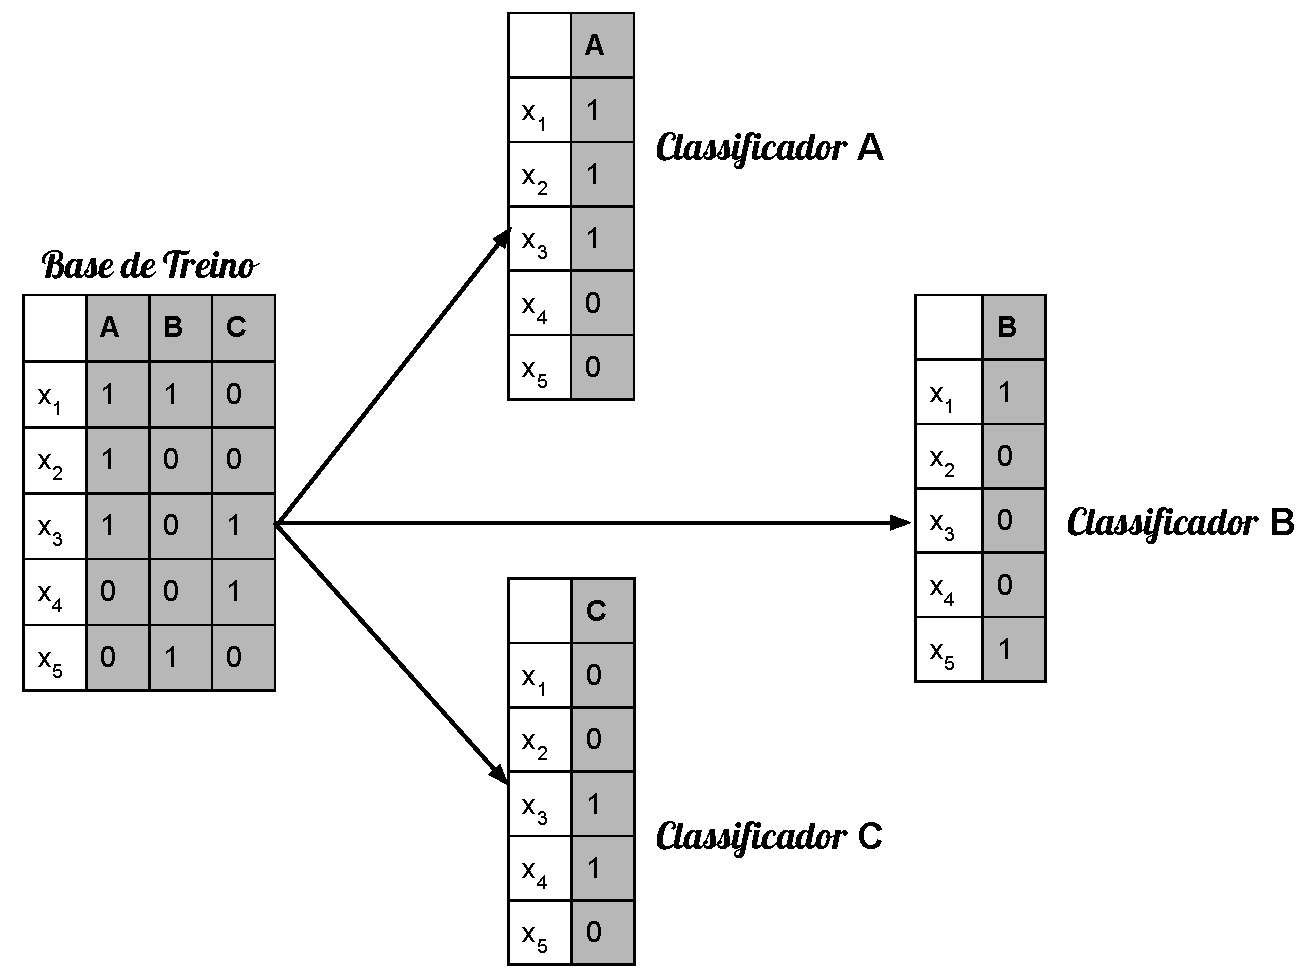
\includegraphics[width=1\linewidth]{BR-figure2}
 
 \caption{Exemplo da transformação realizada pelo método \textit{BR}}
\label{fig:br}

\end{figure}

A figura \ref{fig:br} ilustra um exemplo da transformação que o BR realiza em um problema multirrótulo
de rótulos $A,B$ e $C$ e 6 instâncias. Nele vemos que o BR transforma a base de treino em 3 novas bases
de dados, um para cada classificador binário.





\subsection{Classifier Chain}


A idéia básica desse algoritmo é semelhante ao BR: realiza a transformação do
problema multirrótulo decompondo-o em diversos problemas
de classificação binária unirrótulo, um para cada um dos rótulos do problema.
Ele é também composto de $r$ classificadores binários $c_1,c_2,...,c_r$ e cada um
é associado a um único rótulo distinto. A diferença do \textit{Classifier Chain} para o BR está
em que os classificadores binários estão organizados em uma cadeia de tal forma que
o classificador $c_i$ é contruído com base nos rótulos ou predições dos classificadores anteriores
($c_{i-1},c_{i-2},...,c_{1}$) \cite{cc2009}. O classificador $c_i$ não está necessariamente associado ao rótulo $r_i$,
ele pode estar associado a qualquer um dos rótulos.
Essa associação é feita de forma aleatória ou pré-definida por parâmetro do algoritmo.

Na fase de treinamento do método o espaço de características de cada classificador $c_i$ é 
extendido com os valores dos $i-1$ rótulos reais anteriores da cadeia. Veja um exemplo 
ilustrado na figura \ref{fig:CCtraintest} onde o método é treinado sobre uma base de treino de três rótulos ($A,B,C$)
e seis instâncias. Note que a base de treino do classificador binário $B$ tem como característica adicional o rótulo $A$.

Na fase de predição do método a classificação ocorre de forma sequencial, na ordem em que a cadeia foi definida.
O classificador $c_1$ inicia o processo de classificação realizando a estimativa do rótulo associado da instância teste.
A partir daí o classificador $c_i$ realiza a predição da instância teste assim que a predição do classificador $c_{i-1}$
esteja disponível. O classificador $c_i$ agrega a predição do classificador $c_{i-1}$, que é um valor binário (0 ou 1),
a instância de teste. A figura \ref{fig:CCtraintest} ilutra bem o processo de predição na qual o vetor de características da
instância teste vai crescendo com adição de cada estimativa de rótulo.


\begin{figure}

 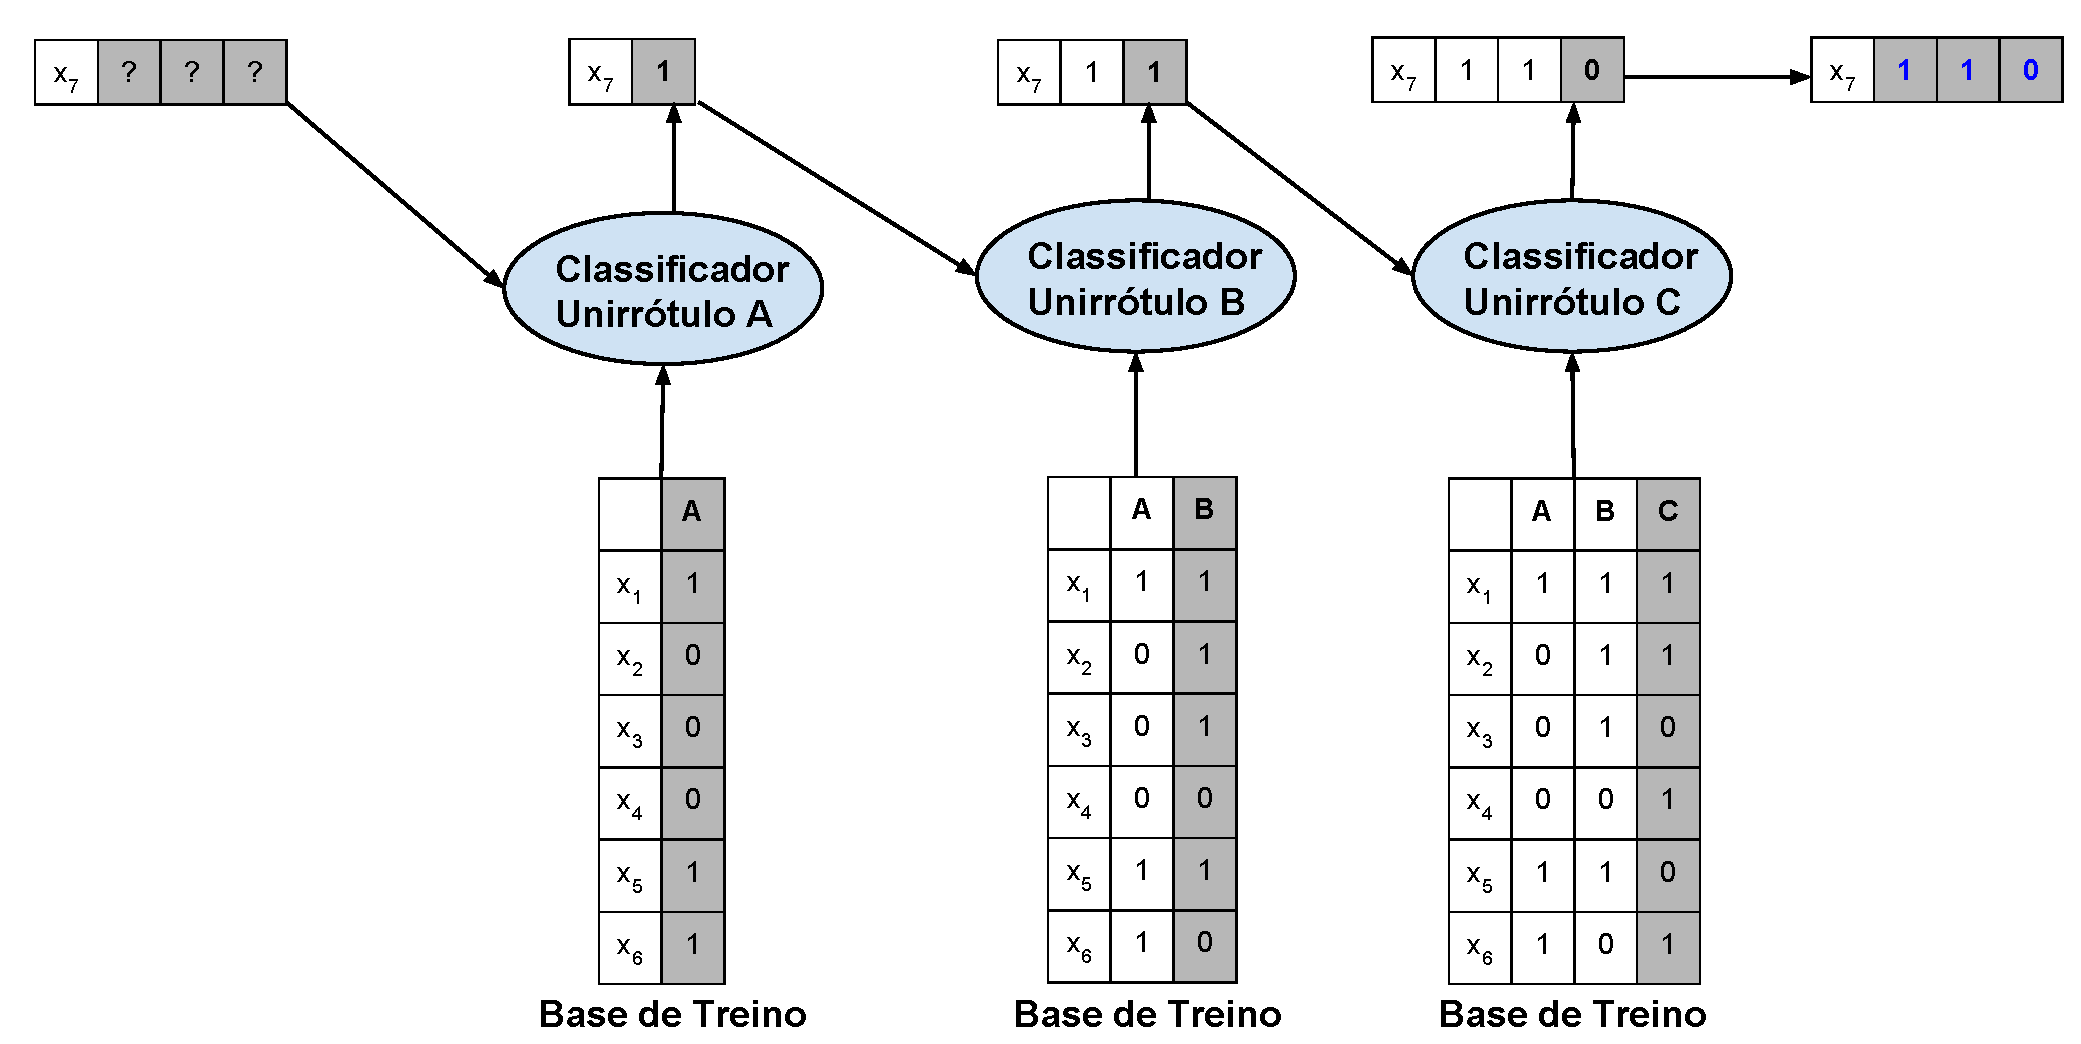
\includegraphics[width=1\linewidth]{CC-train-test}
 \caption{Ilustração de um exemplo da fase de treinamento e de predição do método Classifier Chain.}
\label{fig:CCtraintest}
\end{figure}


\subsection{Ensemble of Classifier Chain}
O \textit{Ensemble of Classifier Chain} é composto de $k$ \textit{Classifiers Chain} distintos \cite{cc2009},
para um $k$ pré-definido.
Para \textit{Classifier Chain} do \textit{Ensemble} é definido uma ordem aleatória da cadeia e
cada \textit{Classifier Chain} é treinado sobre um amostra aleatória da base de dados de treino.
Na fase de predição, a instância de teste é submetida a todos os \textit{Classifiers Chain}, resultando
em $k$ predições para uma mesma instância. A predição única final é uma combinação das $k$ predições individuais,
que é feito por voto majoritário, ou seja, um rótulo $y$ estará na predição final se $y$ estiver
em pelo menos $\ceil{\frac{k}{2}}$ das predições individuais.
O motivo para que cada \textit{Classifier Chain} do \textit{Ensemble} ser diferente é que
ao combinar um classificador $c$ com outros classificadores diferentes,
espera-se que nas instâncias em que as $c$ errar na predição dos rótulos, a maior parte dos outros
classificadores acertem.




\subsection{Relevância Binária Dependente - DBR}
\label{sec:dbr}
Este método é proposto por \cite{dbr2014} é baseado no método BR
e a diferença entre ambos está no fato de 
que o DBR considera dependência entre os $r$ rótulos.

O DBR é composto de dois classificadores multirrótulo, $c_0$ e $c_1$ , 
cada um composto de $r$ classificadores binários. O classificador multirrótulo $c_0$ é
exatamente o método BR. Os $r$ classificadores binários $c_1^1,c_1^2...,c_1^r$ que compoêm $c_1$ 
  trabalham em um novo espaço de características $X^{new}=X \times \{0,1\}^{r-1}$.
  Esse novo espaço é a extensão do antigo com a adição de $r-1$ rótulos.
  Digamos que $(x,y)$ seja uma instância do espaço original $X \times Y$
  onde $x \in X$ e $y \in {\{0,1\}}^{r}$, então cada instância
  do classificador binário $c_1^i$ tem $|x|+r-1$ características
  e é definido como sendo $(x,y_1,...,y_{i-1},y_{i+1},...,y_{r})$.
  
  \subsubsection{Fase de Treinamento}
  Dado uma base de dados de treino $D=\{((x_i),y_i)|i=1,...,n\}$ onde $x_i \in X$ é o vetor de características de cada instância
  e $y_i \in Y$ o vetor binário de rótulos de cada instância,
  primeiro treina-se o $c_0$
  no espaço de características original conforme o treinamento do próprio BR mostrado na seção \ref{sec:br}.
  Depois, treina-se $c_1$ em uma nova base de dados $D'$ que é construída a partir de $D$ adicionando os rótulos de cada
  exemplo como características. Assim, $D'$ é composta pelos exemplos $\{((x_i,y_i),y_i) |i=1,...,n\}$ e
  cada classificador binário $c_1^j$ de $c_1$ é induzido na base de dados $D'_j=\{(x_i,y_{i,1},...,y_{i,j-1},y_{i,j+1},...,y_{i,r}),y_{i,j} | i=1,...,n\}$.
  Note que a característica representando o $j$-ésimo rótulo é removido da base de dados.
  Dessa forma, ao invés de estimar apenas $P(y_j|x)$ como o BR faz, o método é capaz de detectar dependência entre os rótulos ao
  estimar $P(y_j|x,y_1,...,y_{j-1},y_{j+1},...,y_r)$.
  
  \subsubsection{Fase de Predição}
  Como no caso do Classifier Chain, os rótulos reais $y$, que são usado como características adicionais em cada instância de treino,
 estão disponíveis apenas durante a fase de treinamento.
 Com isso, para tornar possível a classificação por $c_1$, o DBR usa o classificador $c_0$ com a finalidade de
 estimar os rótulos, %  Para alcançar isso, o \MRLMa~, após treinado, usa $c_0$ para realizar as primeiras estimativas dos rótulos,
 o que resulta no predição $c_0(x)=\hat{y}=(\hat{y}_1,\hat{y}_2,...,\hat{y}_r)$, que servirá como parte da instância de $c_1$,
 onde antes era o lugar de $y$. 
 A partir daí, $c_1$ classifica o vetor de características $(x,\hat{y})$ de uma forma bem similar ao BR:
 cada classificador binário $c_1^i$ do método é responsável pela predição de um único rótulo da instância
 cujo vetor de características é $(x,\hat{y}_1,...,\hat{y}_{j-1},\hat{y}_{j+1},...,\hat{y}_r)$.

\subsection{Monte Carlo Classifier Chain}


O método \textit{Classifier Chain with Monte Carlo Optimization} (MCC) é introduzido
por \cite{mcc2012} para melhorar a qualidade de predição do \textit{Classifier Chain}.
O método usa uma heurística gulosa para melhorar a fase de predição do \textit{Classifier Chain}.
O método parte do pressuposto de que o \textit{Classifier Chain} geralmente não encontra
o conjunto de rótulos $y^*,y^* \in {\{0,1\}}^r$ que tem a maior probabilidade de a instância de teste ter,
dado o vetor de características da instância, ou seja, não segue corretamente a equação \ref{eq:funcprob}.
Para encontrar o $y^*$ de maior probabilidade, a princípio deve-se procurar entre todas as possíveis
combinações de ${\{0,1\}}^r$, o que torna-se inviável para um valor de $r>10$.
O MCC tenta encontrar esse $y^*$ sem testar todas as possíveis $2^r$ combinações do espaço de busca.
Ele usa de um algoritmo de otimização, chamado \textit{Monte Carlo} \cite{montecarlo}, para
testar apenas algumas dessas combinações.



 

% \section{Adaptação de classificadores}
% \subsection{ML-KNN}
% \subsection{Rede Neural Artificial}
% \subsection{C4.5 multirrótulo}
% \subsection{CRankSVM}
% \subsection{MAIS...}


\chapter{Recursive Dependent Binary Relevance - RDBR}
A proposta de \MRLM~(\MRLMa)~é fundamentada no \MML~\textit{dependent binary relevance} (DBR) \cite{dbr2014}, que é explicado
na seção \ref{sec:dbr}. Assim como o DBR e o CC, o \MRLMa~é um método baseado na transformação do problema que dividem o problema
multirrótulo em vários problemas classificação binária. Todos eles exploram a correlação entre os rótulos por meio da adição de
características especiais que representam os rótulos reais ou estimativas dos rótulos reais ao espaço de características original. 
Mas, diferentemente dos outros, o \MRLMa~adiciona uma inteligência no uso dessas características especiais na fase de predição do método.
A forma de como isso é feito, bem como o funcionamento completo do algoritmo de classificação e a fundamentação teórica
do \MRLMa~são detalhados na seção \ref{sec:mrlm_algo}. 
A seção \ref{sec:mrlm_analise} analisa o funcionamento e o desempenho do \MRLMa~de forma empírica.


\section{Algoritmo de \MRLM~-~\MRLMa}
\label{sec:mrlm_algo}
Como foi dito anteriormente, o \MRLM~é baseado no DBR. 
% Ambos se baseiam na expansão do espaço de características
% com características que representam a estimativas dos rótulos como forma de explorar
% a correlação entre rótulos. Isso é feito usando a predição do BR no espaço de características original.
% Ou seja, 
Ambos dependem da hipótese de que as estimativas dos rótulos em $Y$ por um classificador multirrótulo $c_0$
são boas características para aprimorar as estimativas dos mesmos rótulos por um novo classificador $c_1$
e que quanto melhor forem as estimativas dos rótulos por $c_0$, melhores são as de $c_1$.
% Nesse caso, podemos dizer
% que o classificador $c_0$ é usado por $c_1$ como parâmetro para .
E ainda ambos usam o BR como classificador multirrótulo base, que servirá para realizar as primeiras estimativas dos 
rótulos.

No entanto, o \MRLMa, ao invés de usar apenas o classificador base $c_0$ como função para contruir
as características adicionais que o $c_1$ usa, como o DBR,
ele também usa o próprio $c_1$ para essa finalidade, ou seja, há uma atualização das estimativas das características
pelo próprio classificador que as usam.
A idéia é que cada vez que $c_1$ as atualiza, melhores ficam suas estimativas uma vez que ele será baseado
em estimativas melhores de rótulos do que anteriormente. 
% A alimentação é a propagação das 
% estimativas dos rótulos de um classificador multirrótulo para o espaço de características expandido de um outro, ou o mesmo,
% classificador multirrótulo.
O funcionamento do algoritmo é detalhado nas subseções \ref{sec:mrlm_train} e \ref{sec:mrlm_prediction}.
Formalmente, a estrutura do \MRLMa~é organizado da seguinte forma:
\begin{itemize}
%   \item Assim como o DBR, é composto de dois classificadores multirrotulo, o primeiro, $c_0$, é um BR
%   e o segundo, $c_1$, é um BR ligeiramente modificado, que chamaremos de $BR^*$.
  \item Assim como o DBR, é composto de um BR e um classificador multirrótulo, $c_0$ e $c_1$,
  cada um composto de $r$ classificadores binários.
  \item O $c_0$ trabalha dentro do espaço de características original do problema, de nome $X$,
  e $c_1$ trabalha dentro de um novo espaço de características do problema, de nome $X_e$ e
   definido como $X_e=X \times \{0,1\}^{r}$. Assim, $c_0$ e $c_1$ são
  representados pelas seguintes funções:
  \begin{equation}
  \begin{split}
   & c_0 : X \rightarrow \{0,1\}^r \\
   & c_1 : X_e \rightarrow \{0,1\}^r
   \end{split}
  \end{equation}
  \item Os $r$ classificadores binários $c_1^1,c_1^2...,c_1^r$ que compoêm $c_1$ não trabalham no mesmo
  espaço de características, contudo,
  trabalham com uma dimensão reduzida, em $X \times \{0,1\}^{r-1}$. Digamos que $(x,y)$ seja uma instância de $X_e$
  onde $x \in X$ e $y \in {\{0,1\}}^r$, então cada instância 
  do classificador binário $c_1^i$ tem $|x|+r-1$ características e é definido como sendo $(x,y_1,...,y_{i-1},y_{i+1},...,y_{r})$.

  
%   e o resultado da classificação multirrotulo de $c_1$ é construido da seguinte forma:
%   $c_0(x,y)=(c_1^1(x,y_2$
%   \item O método contém duas funções $t_0$ e $t_1$ que mapeiam espaços de características:
%    \begin{equation}
%  \begin{split}
%     & t_0 : X \rightarrow X_e \\
%     & t_1 : X_e \rightarrow X_e \\
%     & t_0(x)=(c_0(x)) | x \in X \\
%     & t_1(x,y)=(c_1(x,y)) | x \in X,  y \in [0,1]^{l}
% %   h_i : \mathbb{R}^l \rightarrow \mathbb{R}^l & | i=1,...,n-1
%   \end{split}
%  \end{equation}
%   
  
\end{itemize}
  As seções seguintes explicam o funcionamento da estrutura apresentada 
  bem como formalizam e detalham tanto a fase de treinamento quanto a fase de predição do algoritmo.
  É importante observar que a fase de treinamento do \MRLMa~é exatamente o mesmo do que o DBR.
  A diferença de ambos os métodos se dá na fase de predição, descrita na seção \ref{sec:mrlm_prediction}.
 
 
 \subsection{Fase de Treinamento}
 \label{sec:mrlm_train}
  A fase de treinamento do \MRLMa~é exatamente igual ao DBR.
  
  Formalmente, o treinamento de \MRLM~funciona da seguinte forma.
  Dado uma base de dados de treino $D=\{((x_i),y_i)|i=1,...,n\}$ onde $x_i \in X$ é o vetor de características de cada instância
  e $y_i \in Y$ o vetor binário de rótulos de cada instância,
  primeiro treina-se o $c_0$
  no espaço de características original conforme o treinamento do próprio BR mostrado na seção \ref{sec:br}.
%   Depois, treina-se $c_1$ em uma nova base de dados $D'$ que é construída a partir de $D$ e que é
%   composta pelas instâncias $\{(y_1),(y_2),...,(y_n)\}$ as quais são os rótulos das instâncias da base de $D$
%   (ver figura \ref{fig:instsRotulos}).
  Depois, treina-se $c_1$ em uma nova base de dados $D'$ que é construída a partir de $D$ adicionando os rótulos de cada
  exemplo como características. Assim, $D'$ é composta pelos exemplos $\{((x_i,y_i),y_i) |i=1,...,n\}$ e
  cada classificador binário $c_1^j$ de $c_1$ é induzido na base de dados $D'_j=\{(x_i,y_{i,1},...,y_{i,j-1},y_{i,j+1},...,y_{i,r}),y_{i,j} | i=1,...,n\}$.
  Note que a característica representando o $j$-ésimo rótulo é removido da base de dados.
  Dessa forma, ao invés de estimar apenas $P(y_j|x)$ como o BR faz, o método é capaz de detectar dependência entre os rótulos ao
  estimar $P(y_j|x,y_1,...,y_{j-1},y_{j+1},...,y_r)$.
 
 \subsection{Fase de Predição}
 \label{sec:mrlm_prediction}
 O funcionamento do \MRLMa~distingue-se do DBR apenas na fase de predição.
 Dado o vetor de características $x$ de uma instância 
 onde $x\in X$ e seu conjunto de rótulos reais $y,y \in {\{0,1\}}^r$, queremos que a função $C:X\rightarrow Y$,
 representando o classificador multirrótulo \MRLMa, retorne $y$ quando o submetemos $x$, ou seja, $C(x)=y$.
 
 Como no caso do DBR e do Classifier Chain, os rótulos reais $y$, que são usado como características especiais,
 estão disponíveis apenas durante a fase de treinamento. Dessa forma, para tornar possível a classificação por $c_1$, usou-se o $c_0$ para
 estimar os rótulos, %  Para alcançar isso, o \MRLMa~, após treinado, usa $c_0$ para realizar as primeiras estimativas dos rótulos,
 resultando em $c_0(x)=\hat{y}^0=(\hat{y}_1^0,\hat{y}_2^0,...,\hat{y}_r^0)$, que servirá como parte da instância de $c_1$
 no lugar de $y$. 
A partir daí, $c_1$ classifica o vetor de características $(x,\hat{y}^0)$ de uma forma bem similar ao BR:
 cada classificador binário $c_1^i$ do método é responsável pela predição de um único rótulo da instância
 cujo vetor de características é $(x,\hat{y}_1^0,...,\hat{y}_{j-1}^0,\hat{y}_{j+1}^0,...,\hat{y}_r^0)$. 
 Esse procedimento é o realizado pelo DBR e é ilustrado na figura \ref{fig:DBRstruct}. 
 Nela vemos quais estimativas de rótulos são utilizadas como características adicionais para classificação final
 de uma instância.
 
   \begin{figure}
\centering
$
\psmatrix[colsep=.6cm,rowsep=.4cm,linewidth=.4pt]
\\
\\
& \bigcirc &\circ&&\bigcirc&\enspace&\\
&\vdots\\
& \bigcirc &\circ&&\bigcirc&\enspace&\\
&\vdots\\
& \bigcirc &\circ&&\bigcirc&\enspace&\\
&\mathrm{BR}&&&\mathrm{DBR}
\ncline[linestyle=dotted]{3,3}{3,5}
\ncput*[npos=.65]{\|}
\ncline[linestyle=dotted]{5,3}{5,5}
\ncput*[npos=.65]{\|}
\ncline[linestyle=dotted]{7,3}{7,5}
\ncput*[npos=.65]{\|}
\ncline{->}{3,2}{3,3}
\ncline{->}{5,2}{5,3}
\ncline{->}{7,2}{7,3}
\ncline{->}{3,3}{5,5}
\ncline{->}{3,3}{7,5}
\ncline{->}{5,3}{3,5}
\ncline{->}{5,3}{7,5}
\ncline{->}{7,3}{3,5}
\nccircle[linestyle=none]{3,3}{.01cm}_{\hat{y}_1}
\nccircle[linestyle=none]{5,3}{.01cm}_{\hat{y}_j}
\nccircle[linestyle=none]{7,3}{.01cm}_{\hat{y}_r}
\nccircle[linestyle=none]{3,6}{.01cm}_{\hat{y}_1}
\nccircle[linestyle=none]{5,6}{.01cm}_{\hat{y}_j}
\nccircle[linestyle=none]{7,6}{.01cm}_{\hat{y}_r}
\ncline[arm=50pt]{->}{7,3}{5,5}
\ncline{->}{3,5}{3,6}
\ncline{->}{5,5}{5,6}
\ncline{->}{7,5}{7,6}
\nccircle[linestyle=none]{3,5}{.12cm}>{ c_1^0 }
\nccircle[linestyle=none]{5,5}{.12cm}>{ c_1^j }
\nccircle[linestyle=none]{7,5}{.12cm}>{ c_1^r }
\nccircle[linestyle=none]{3,2}{.12cm}>{ c_0^0 }
\nccircle[linestyle=none]{5,2}{.12cm}>{ c_0^j }
\nccircle[linestyle=none]{7,2}{.12cm}>{ c_0^r }
\endpsmatrix
$
\caption{Arquitetura do classificador \textit{Dependent Binary Relevance} (DBR).
Na primeira camada (a esquerda), os classificadores binários do BR proveem cada
um dos rótulos individualmente. A próxima camada provê a estimativa final dos rótulos.}
\label{fig:DBRstruct}
\end{figure}
 
   \begin{figure}
\centering
$
\psmatrix[colsep=.6cm,rowsep=.4cm,linewidth=.4pt]
\\
\\
& \bigcirc &\circ&&\bigcirc&\circ&\\
&\vdots\\
& \bigcirc &\circ&&\bigcirc&\circ&\\
&\vdots\\
& \bigcirc &\circ&&\bigcirc&\circ&\\
&\mathrm{BR}&&&\mathrm{RDBR}
\ncline[linestyle=dotted]{3,3}{3,5}
\ncput*[npos=.65]{\|}
\ncline[linestyle=dotted]{5,3}{5,5}
\ncput*[npos=.65]{\|}
\ncline[linestyle=dotted]{7,3}{7,5}
\ncput*[npos=.65]{\|}
\ncline{->}{3,2}{3,3}
\ncline{->}{5,2}{5,3}
\ncline{->}{7,2}{7,3}
\ncline{->}{3,3}{5,5}
\ncline{->}{3,3}{7,5}
\ncline{->}{5,3}{3,5}
\ncline{->}{5,3}{7,5}
\ncline{->}{7,3}{3,5}
\nccircle[linestyle=none]{3,3}{.01cm}_{\hat{y}_1}
\nccircle[linestyle=none]{5,3}{.01cm}_{\hat{y}_j}
\nccircle[linestyle=none]{7,3}{.01cm}_{\hat{y}_r}
\nccircle[linestyle=none]{3,6}{.01cm}_{\hat{y}_1}
\nccircle[linestyle=none]{5,6}{.01cm}_{\hat{y}_j}
\nccircle[linestyle=none]{7,6}{.01cm}_{\hat{y}_r}
\ncline[arm=50pt]{->}{7,3}{5,5}
\ncline{->}{3,5}{3,6}
\ncline{->}{5,5}{5,6}
\ncline{->}{7,5}{7,6}
\ncloop[arm=.7,loopsize=0,angleA=90,angleB=90]{->}{3,6}{3,3}
\ncloop[arm=.7,loopsize=0,angleA=90,angleB=90]{->}{5,6}{5,3}
\ncloop[arm=.7,loopsize=0,angleA=90,angleB=90]{->}{7,6}{7,3}
\nccircle[linestyle=none]{3,5}{.12cm}>{ c_1^0 }
\nccircle[linestyle=none]{5,5}{.12cm}>{ c_1^j }
\nccircle[linestyle=none]{7,5}{.12cm}>{ c_1^r }
\nccircle[linestyle=none]{3,2}{.12cm}>{ c_0^0 }
\nccircle[linestyle=none]{5,2}{.12cm}>{ c_0^j }
\nccircle[linestyle=none]{7,2}{.12cm}>{ c_0^r }
\ncline{->}{3,6}{3,7}
\ncline{->}{5,6}{5,7}
\ncline{->}{7,6}{7,7}
\endpsmatrix
$
\caption{ Arquitetura do \textit{Recursive Dependent Binary Relevance} (RDBR).
Na primeira camada (a esquerda), os classificadores binários do BR proveem estimativas de cada
um dos rótulos individualmente. A próxima camada provê as estimativas obtidas pelo DBR as quais
são usados recursivamente ao realimentar o DBR.
% The realimentation to obtain $\hat{\yy}^{\mathrm{(\tau+1)}}$
% is only performed when the complete estimated
% label vector from the current iteration $\hat{\yy}^{\mathrm{(\tau+1)}}$
% has been calculated.
}
\label{fig:RDBRbatch}
\end{figure}
 
 
%  \begin{equation}
%   c_1(x)=(c_1^1(x),c_1^2(x),...,c_1^l(x))
%  \end{equation}
 
 \begin{figure}
\centering
$
\psmatrix[colsep=.6cm,rowsep=.4cm,linewidth=.4pt]
&\bigcirc&\|&\bigcirc\\
\\
&\bigcirc&\|&\bigcirc\\
\enspace&\enspace&\enspace&\enspace&\enspace\\
\\
&\bigcirc&\|&\bigcirc\\
\\
&\bigcirc&\|&\bigcirc\\
\ncline{->}{1,2}{3,4}
\ncline{->}{3,2}{1,4}
\ncline[linestyle=dotted]{1,2}{1,3}
\ncline[linestyle=dotted]{3,2}{3,3}
\nccircle[linestyle=none]{1,2}{.1cm}^{ y_i^{\mathrm{(\tau)}} }
\nccircle[linestyle=none]{1,4}{.1cm}^{ y_i^{\mathrm{(\tau+1)}} }
\nccircle[linestyle=none]{3,2}{.1cm}^{ y_j^{\mathrm{(\tau)}} }
\nccircle[linestyle=none]{3,4}{.1cm}^{ y_j^{\mathrm{(\tau+1)}} }
\ncline{4,1}{4,5}
\ncline{->}{6,2}{8,4}
\ncline{->}{8,4}{6,4}
\ncline[linestyle=dotted]{6,2}{6,3}
\ncline[linestyle=dotted]{8,2}{8,3}
\nccircle[linestyle=none]{6,2}{.05cm}^{ y_i^{\mathrm{(\tau)}} }
\nccircle[linestyle=none]{6,4}{.05cm}^{ y_i^{\mathrm{(\tau+1)}} }
\nccircle[linestyle=none]{8,2}{.1cm}^{ y_j^{\mathrm{(\tau)}} }
\nccircle[linestyle=none]{8,4}{.1cm}^{ y_j^{\mathrm{(\tau+1)}} }
\endpsmatrix
$
\caption{Estrutura do RDBR com atualização estática (imagem acima) 
e dinâmica (imagem abaixo) dos rótulos.
Na atualização dinâmica, a estimativa dos rótulos $\hat{y_{i}}^{\mathrm{(\tau+1)}}$
é baseado nas estimativas dos rótulos anteriores (da iteração $\mathrm{(\tau)}$)
e nas da iteração atual ($\mathrm{(\tau+1)}$), se
disponíveis.
% 
% 
% Basic idea of the recursive dependent binary relevance
% classifier (RDBR), stochastic version.
% In the upper part the update strategy of the batch version is shown.
% A label $\hat{y_{i}}^{\mathrm{(\tau+1)}}$ is estimated,
% based exclusively on the label
% estimates of the previous estimates $\hat{y_{j}}^{\mathrm{(\tau)}}$.
% In the lower part the update strategy of the stochastic version is shown.
% A label $\hat{y_{i}}^{\mathrm{(\tau+1)}}$ is estimated,
% based on the label estimates of the previous estimates
% and on the current estimates $\hat{y_{j}}^{\mathrm{(\tau+1)}}$,
% as soon as they become available.
}
\label{fig:RDBRstochastic}
\end{figure}

 Assim que $c_1$ classifica a instância $(x,\hat{y}^0)$, gerando portanto a estimativa de rótulos $\hat{y}^1=c_1(x,\hat{y}^0)$,
 $\hat{y}^1$ é usado para atualizar as características da instância $x$, tomando assim o lugar de $\hat{y}^0$.
 Esse processo de atualização das características é iterativo e é repetido $k$ vezes,
 onde $k$ é determinado por um valor máximo de iterações, definido a priori, ou quando é detectado a convergência.
 A convergência é alcançada quando a estimativa de rótulos não muda, independente do número de iterações.
%  Isso acontece, por exemplo, quando $c_1(c_1(c_0))=c_1(c_0)$.
 Com $k$ iterações, tem-se $k$ estimativas de rótulos $\hat{y}^1,\hat{y}^2,...,\hat{y}^k$, dentre as quais o último ($\hat{y}^k$)
 é a classificação final do método $C(x)=\hat{y}^k$.
 
 Dessa forma, podemos concluir que \MRLM~é um método recursivo de tal forma que
 para $k=1$, $C(x)=c_1(x,c_0(x))$,
 para $k=2$, $C(x)=c_1(x,c_1(x,c_0(x)))$,
 para $k=3$, $C(x)=c_1(x,c_1(x,c_1(x,c_0(x))))$ e assim por diante.
 Note que para $k=0$, o \MRLMa~é exatamente o BR, $C(x)=c_0(x)$.
%  a aplicação de $c_1$ $3$ vezes sobre
%  $c_0(x)$ resulta na estimativa $\hat{y}^3=c_1(c_1(c_1(c_0(x))))$ e assim por diante.
 Aplicando esse processo recursivo, espera-se que a cada recursão $i$ a estimativa dos rótulos $\hat{y}^i$ seja melhor do que
 seu antecessor $\hat{y}^{i-1}$. Teoricamente, essa afirmação se mantém se supormos que a estimativa $\hat{y}^1$ é melhor do que a $\hat{y}^0$, 
 o que é razoável uma vez que o classificador $c_0$, que é um BR, obtem seu resultado usando apenas estimativas marginais dos rótulos,
 %  ($P(y|x)=\prod_{j=1}^l{P(y_j,x)}$)
  enquanto que $c_1$ explora a correlação dos rótulos ao usá-los como características, obtendo assim 
 estimativas baseadas na probabilidade condicional.
 Com essa suposição teríamos que $\hat{y}^i$ seria melhor do que $\hat{y}^{i-1}$, pois $\hat{y}^{i-1}$ se aproxima
 mais da distribuição real dos rótulos do que $\hat{y}^{i-2}$. Assim, quando $c_1$ estimar $\hat{y}^i$ usando $\hat{y}^{i-1}$ estaria baseado em 
 uma distribuição mais próxima daquela em que foi treinado do que usando $\hat{y}^{i-2}$.
 Lembrando que $c_1$ foi treinado usando apenas rótulos assumidamente corretos.
  Olhando por todo o procedimento descrito, o \MRLMa~pode ser simplesmente visto como uma generalização do BR e do DBR
 que insere uma inteligência
 adicional a aplicação e uso do classificador $c_1$ de DBR, afim de que ele seja melhor aproveitado.
 A figura \ref{fig:RDBRbatch} ilustra bem o funcionamento do RDBR.
 Nela vemos quais estimativas de rótulos são utilizadas como características adicionais
 para próxima estimativa de rótulos.
 
  Adicionalmente, o \MRLMa~adota uma técnica extra, inspirada no Classifier Chain que consiste em, para
 cada classificador binário $c_1^j$, atualizar a característica $\hat{y}_j$ imediatamente após 
 a sua classificação. Dessa forma, os classificadores binários seguintes, $c_1^{j+1},c_1^{j+2},...,c_1^{r}$,
 classificarão suas instâncias baseados em estimativas de rótulos mais atuais, possivelmente melhores. Isso é ilustrado
 na figura \ref{fig:RDBRstochastic} e é chamado de atualização dinâmica dos rótulos.
 

 
 \section{Análise}
 \label{sec:mrlm_analise} 
 
 Nessa seção o método \MRLMa~é posto em prova. Com objetivo de analisar o método, implementou-se o algoritmo
 na linguagem de programação Java e no Weka \cite{weka}, que é uma biblioteca que integra técnicas de reconhecimento de padrões.
 A principal hipótese em que o \MRLMa~é baseado será testado nessa seção com o intuito de validar o método.
 Com a finalidade de tornar os testes mais objetivos, a hipótese é melhor formalizado assim:
 \begin{itemize}

  \item Dados uma métrica $M$, uma base de Teste $D=\{x_1,x_2,...,x_n\}$,
  um DBR induzido composto pelos classificadores multirrótulos $c_0$ e $c_1$ e
  dois vetores de predições de $r$ rótulos:
  \begin{equation}
  \begin{split}
  & p=(p_1,p_2,...,p_n) : p_i \in {\{0,1\}}^r |1 \leq i \leq n \\
  & b=(b_1,b_2,...,b_n) : b_i \in {\{0,1\}}^r |1 \leq i \leq n
  \end{split}
  \end{equation}
  tal que $M(p_2) \geq M(p_1)$,
  então:
  \begin{equation}
  M((c_1(x_i,p_1) | 1 \leq i \leq n)) \leq M((c_1(x_i,p_2) | 1 \leq i \leq n))
  \end{equation}
 
 \end{itemize}

Resumidamente, a hipótese é que erros de predições pelo
classificador $c_0$ do DBR afetam negativamente a classificação do classificador $c_1$.
A comprovação dessa hipótese é feita da seguinte forma. Experimentos com o \MRLMa~são realizados
usando 7 bases de dados de domínio públicos. Cada experimento consiste em medir o valor da métrica \textit{Subset Accuracy}
quando o método é submetido a validação cruzada de 10 \textit{folds}.
O experimento é repetido com o número máximo de iterações do
\MRLMa~variando de 0 a 10 (Note que para o valor 0, o \MRLMa~se torna exatamente o BR).
Ao variar esse parâmetro, espera-se que o método obtenha desempenho melhor para os valores mais altos.
De fato, é o que ocorre na maioria dos casos, apesar de que o método estabiliza/converge rapidamente em relação ao
número de iterações.
Os gráficos da figura \ref{fig:mrlmgraph1} mostram o que ocorre em 5 dos 7 casos testados: o método tem seu desempenho melhorado
até o valor máximo de iterações chegar a 2, depois disso o método não tem seu desempenho alterado.
Portanto 2 foi o valor máximo de iterações necessárias para o método convergir nesses casos.
Nos outros dois casos o método convergiu com apenas uma iteração ou piorou 
com duas ou mais iterações. Veja os dois gráficos dos dois casos na figura \ref{fig:mrlmgraph2}.
Vale ressaltar que em 6 dos 7 casos, o método \MRLMa~conseguiu um desempenho melhor do que o DBR e em apenas um dos casos
alcançou o mesmo desempenho do DBR.



\begin{figure}
\centering
\begin{subfigure}{.5\textwidth}
  \centering
  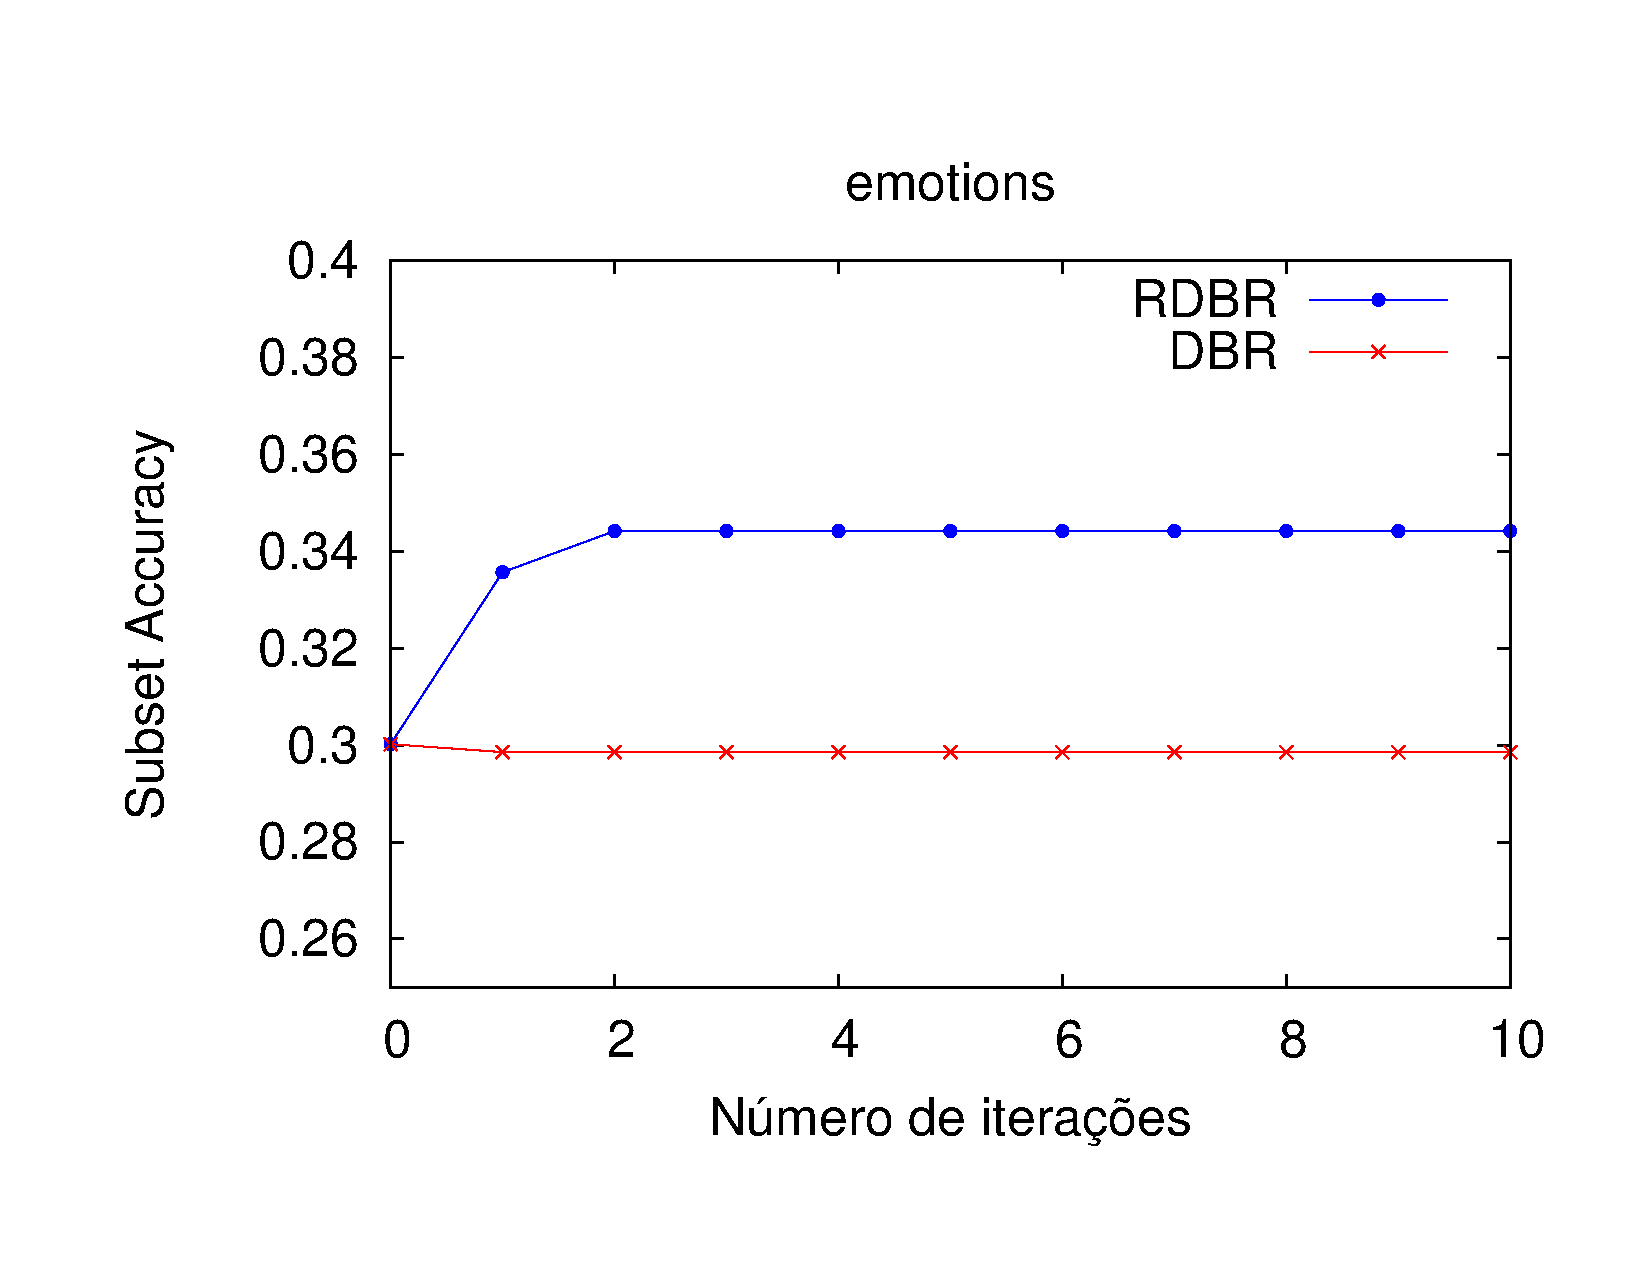
\includegraphics[angle=-90, width=1\linewidth]{plots/emotions.pdf}
  \caption{Emotions}
  \label{fig:subemotions}
\end{subfigure}%
\begin{subfigure}{.5\textwidth}
  \centering
  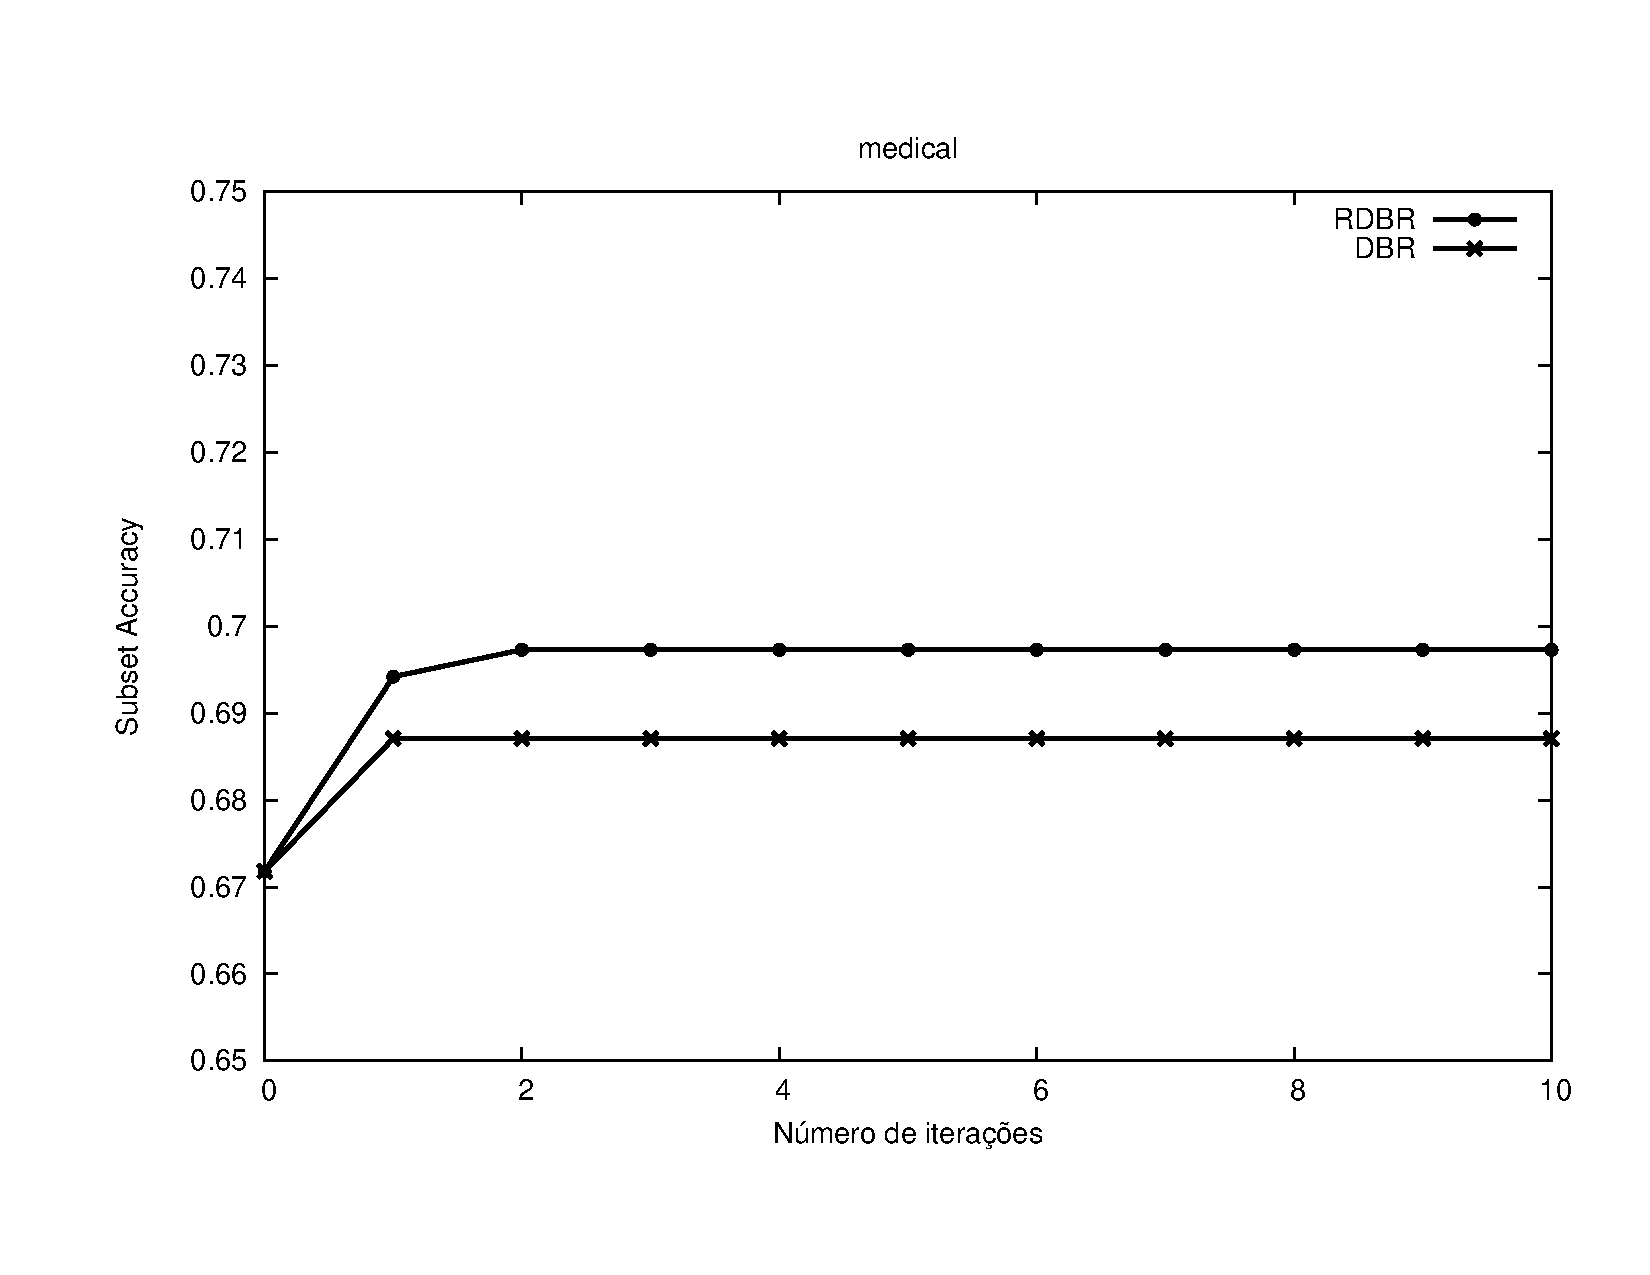
\includegraphics[angle=-90, width=1\linewidth]{plots/medical.pdf}
  \caption{Medical}
  \label{fig:submedical}
\end{subfigure}

\begin{subfigure}{.5\textwidth}
  \centering
  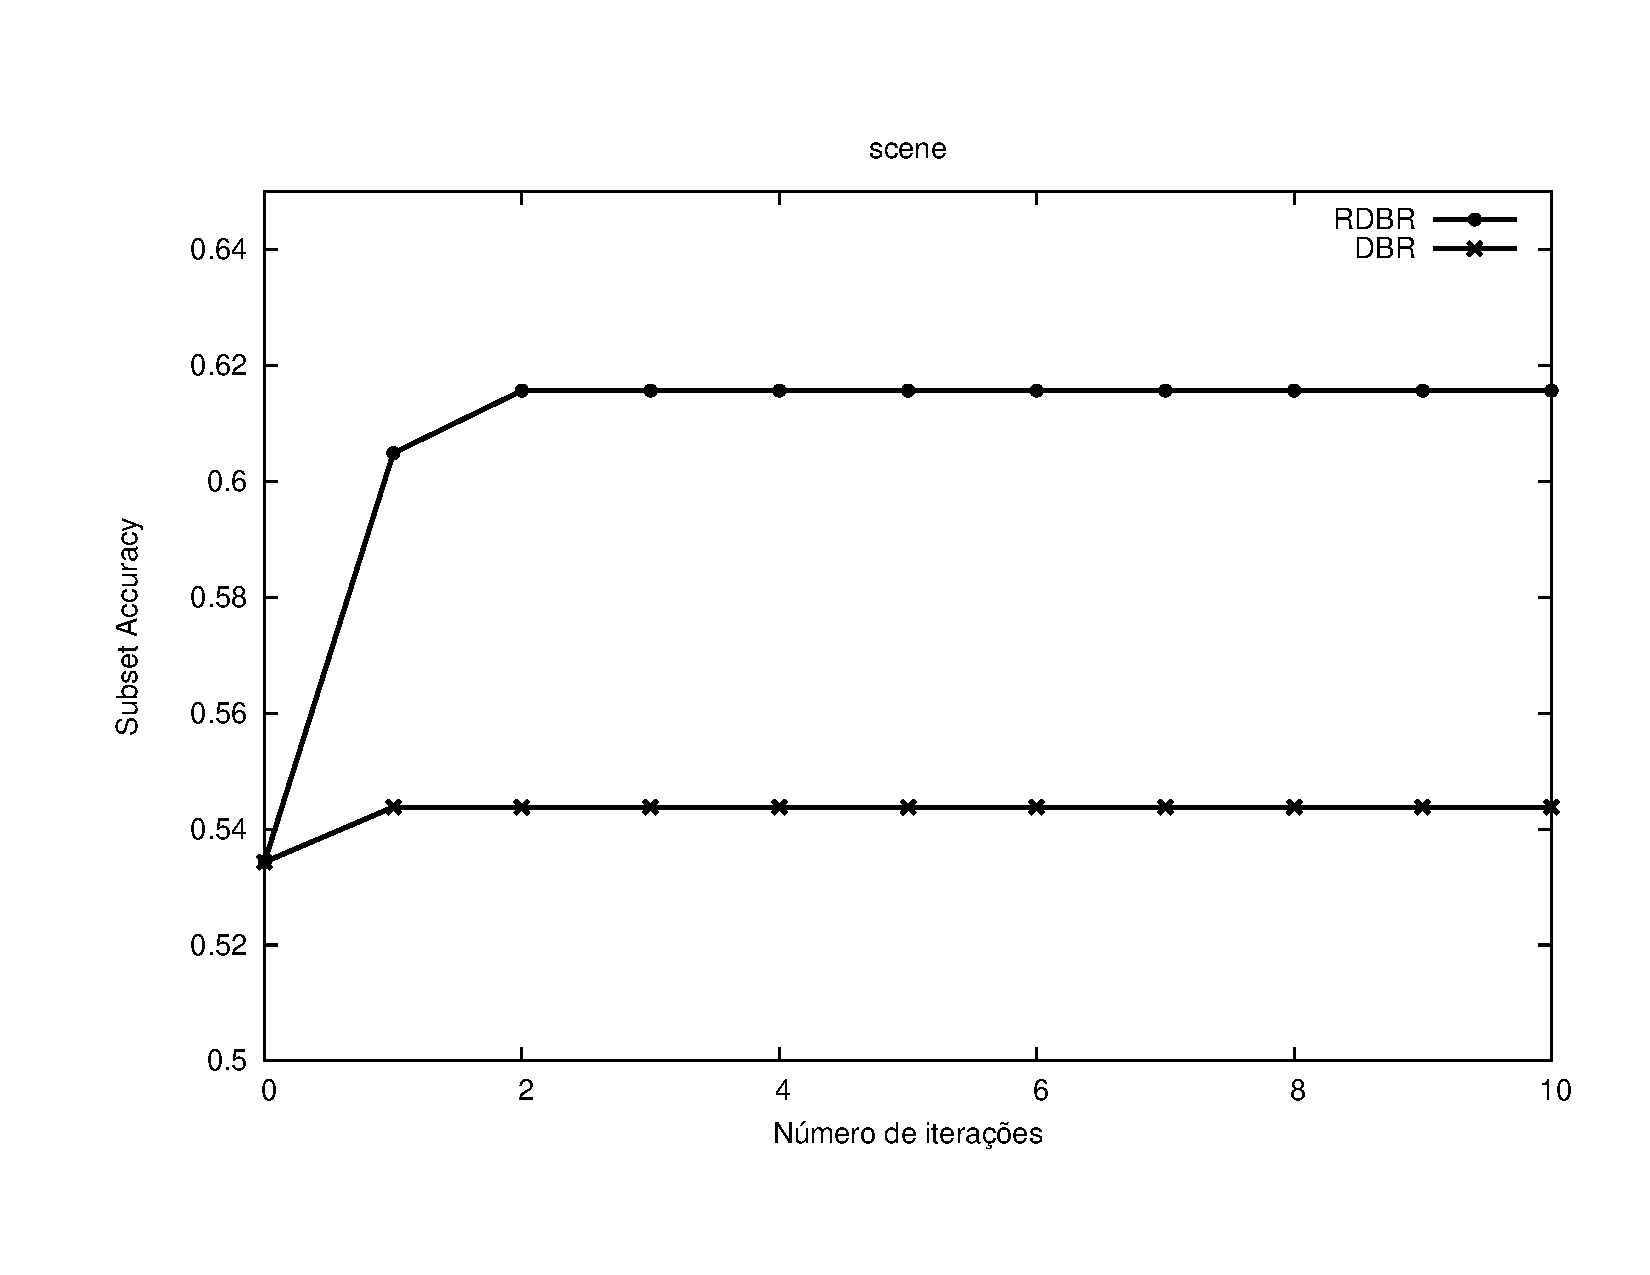
\includegraphics[angle=-90, width=1\linewidth]{plots/scene.pdf}
  \caption{Scene}
  \label{fig:subscene}
\end{subfigure}%
\begin{subfigure}{.5\textwidth}
  \centering
  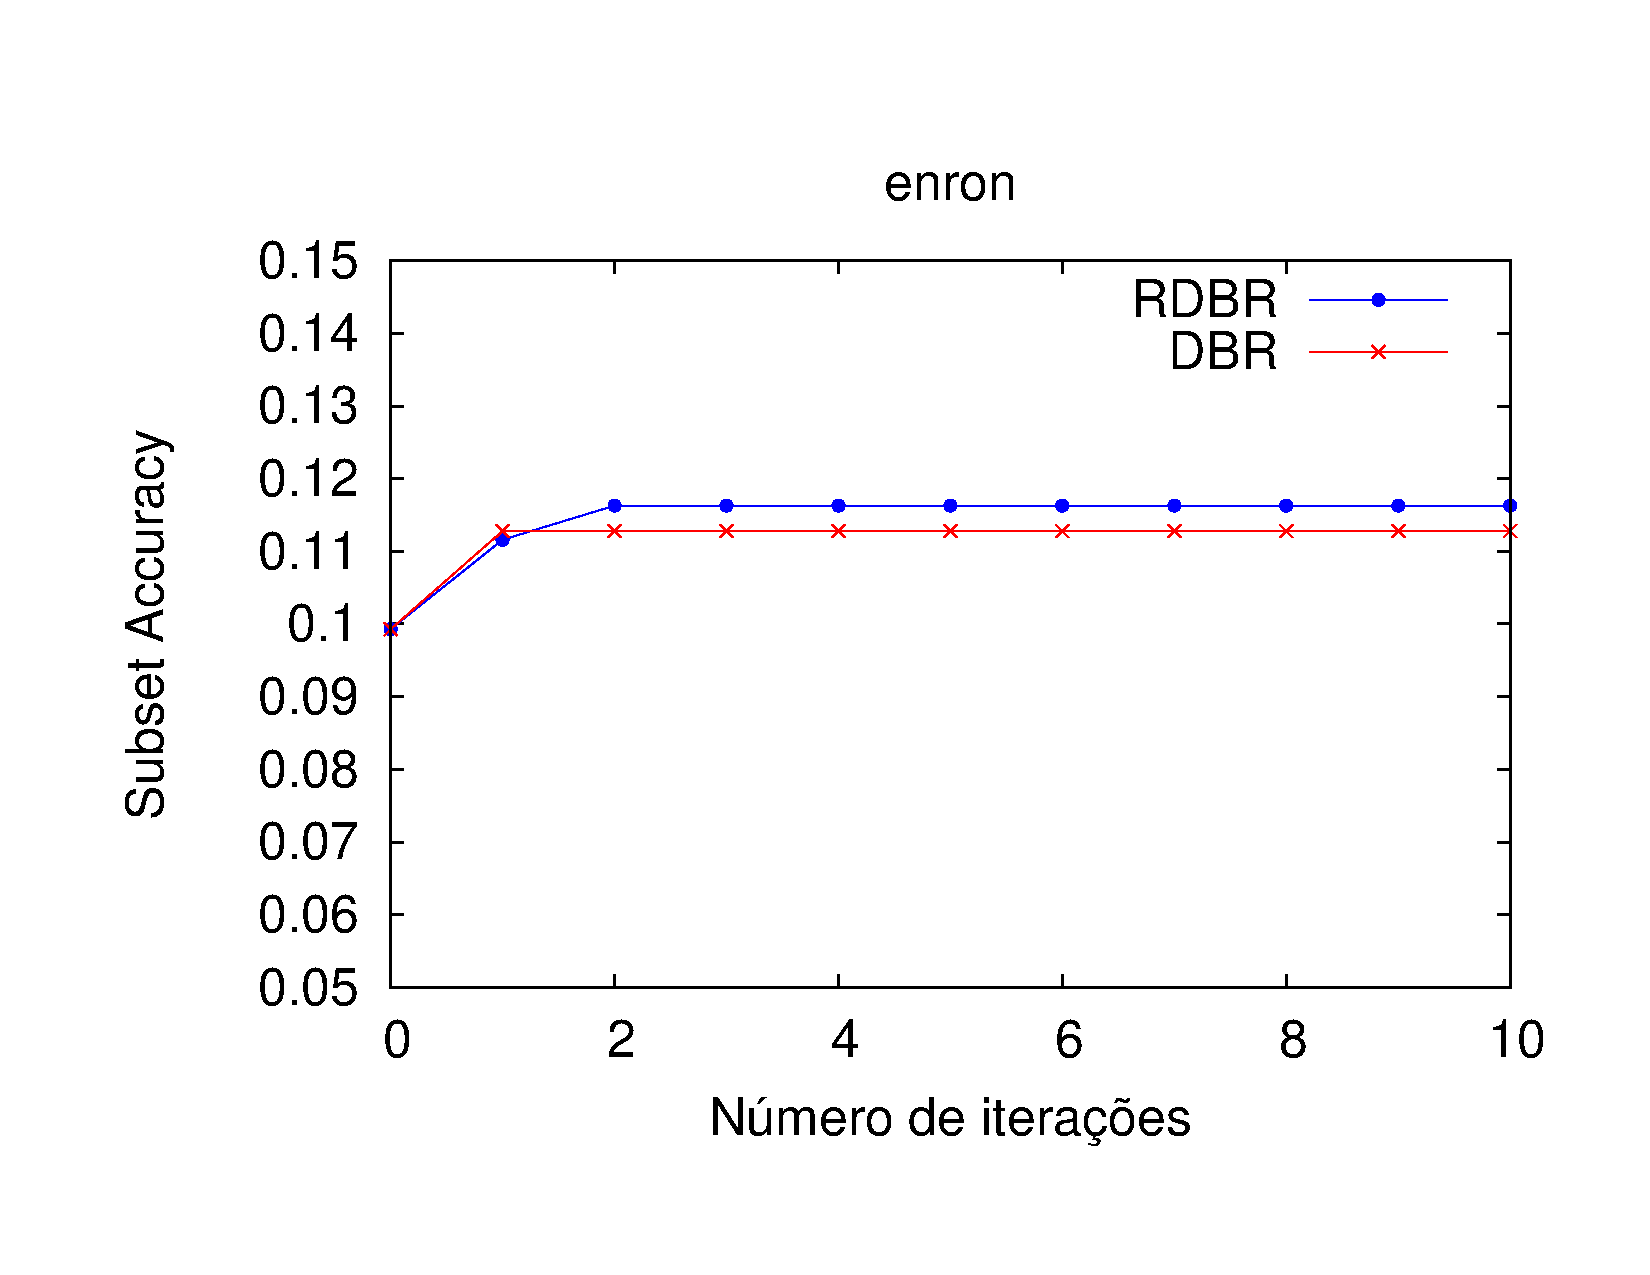
\includegraphics[angle=-90, width=1\linewidth]{plots/enron.pdf}
  \caption{Enron}
  \label{fig:subenron}
\end{subfigure}

\begin{subfigure}{.5\textwidth}
  \centering
  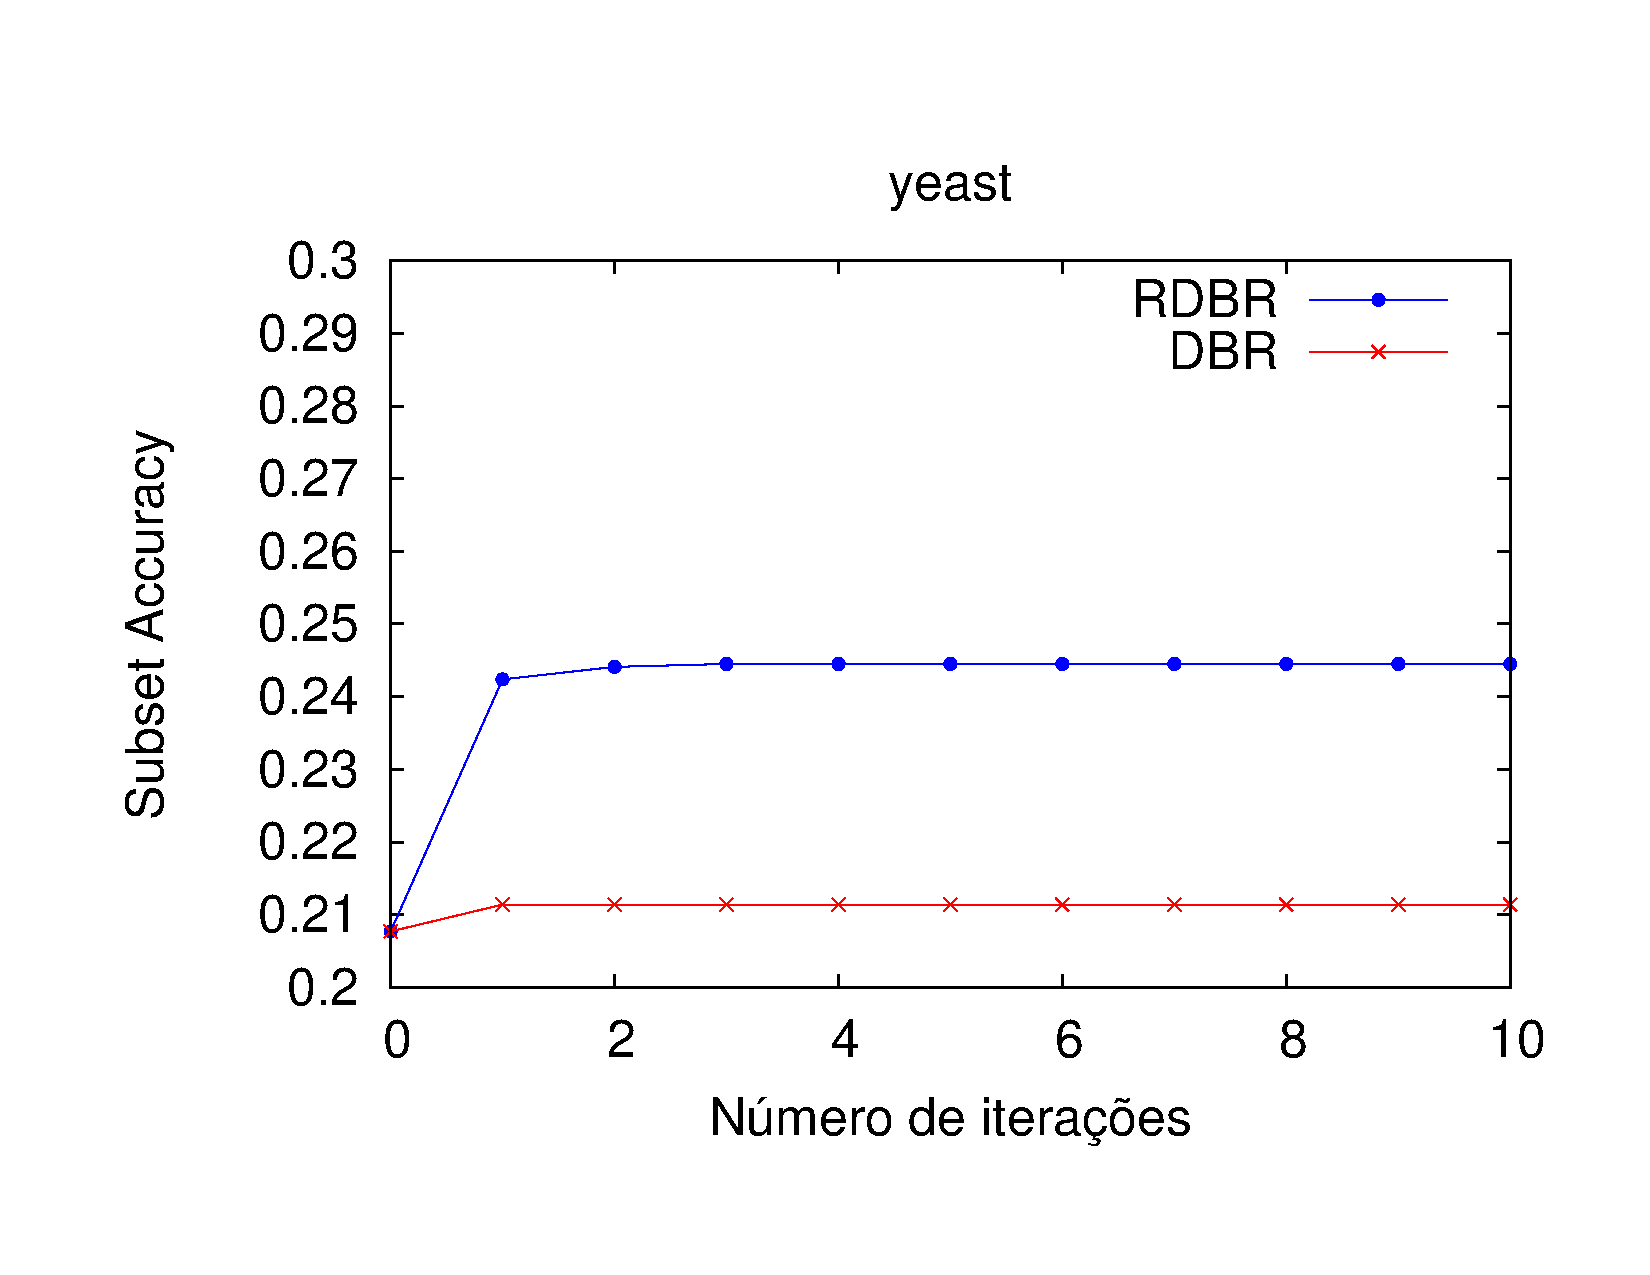
\includegraphics[angle=-90, width=1\linewidth]{plots/yeast.pdf}
  \caption{Yeast}
  \label{fig:subyeast}
\end{subfigure}
\caption{Gráficos de análise de desempenho do \MRLMa.}
\label{fig:mrlmgraph1}
\end{figure}

\begin{figure}
\centering
 \begin{subfigure}{.5\textwidth}
  \centering
  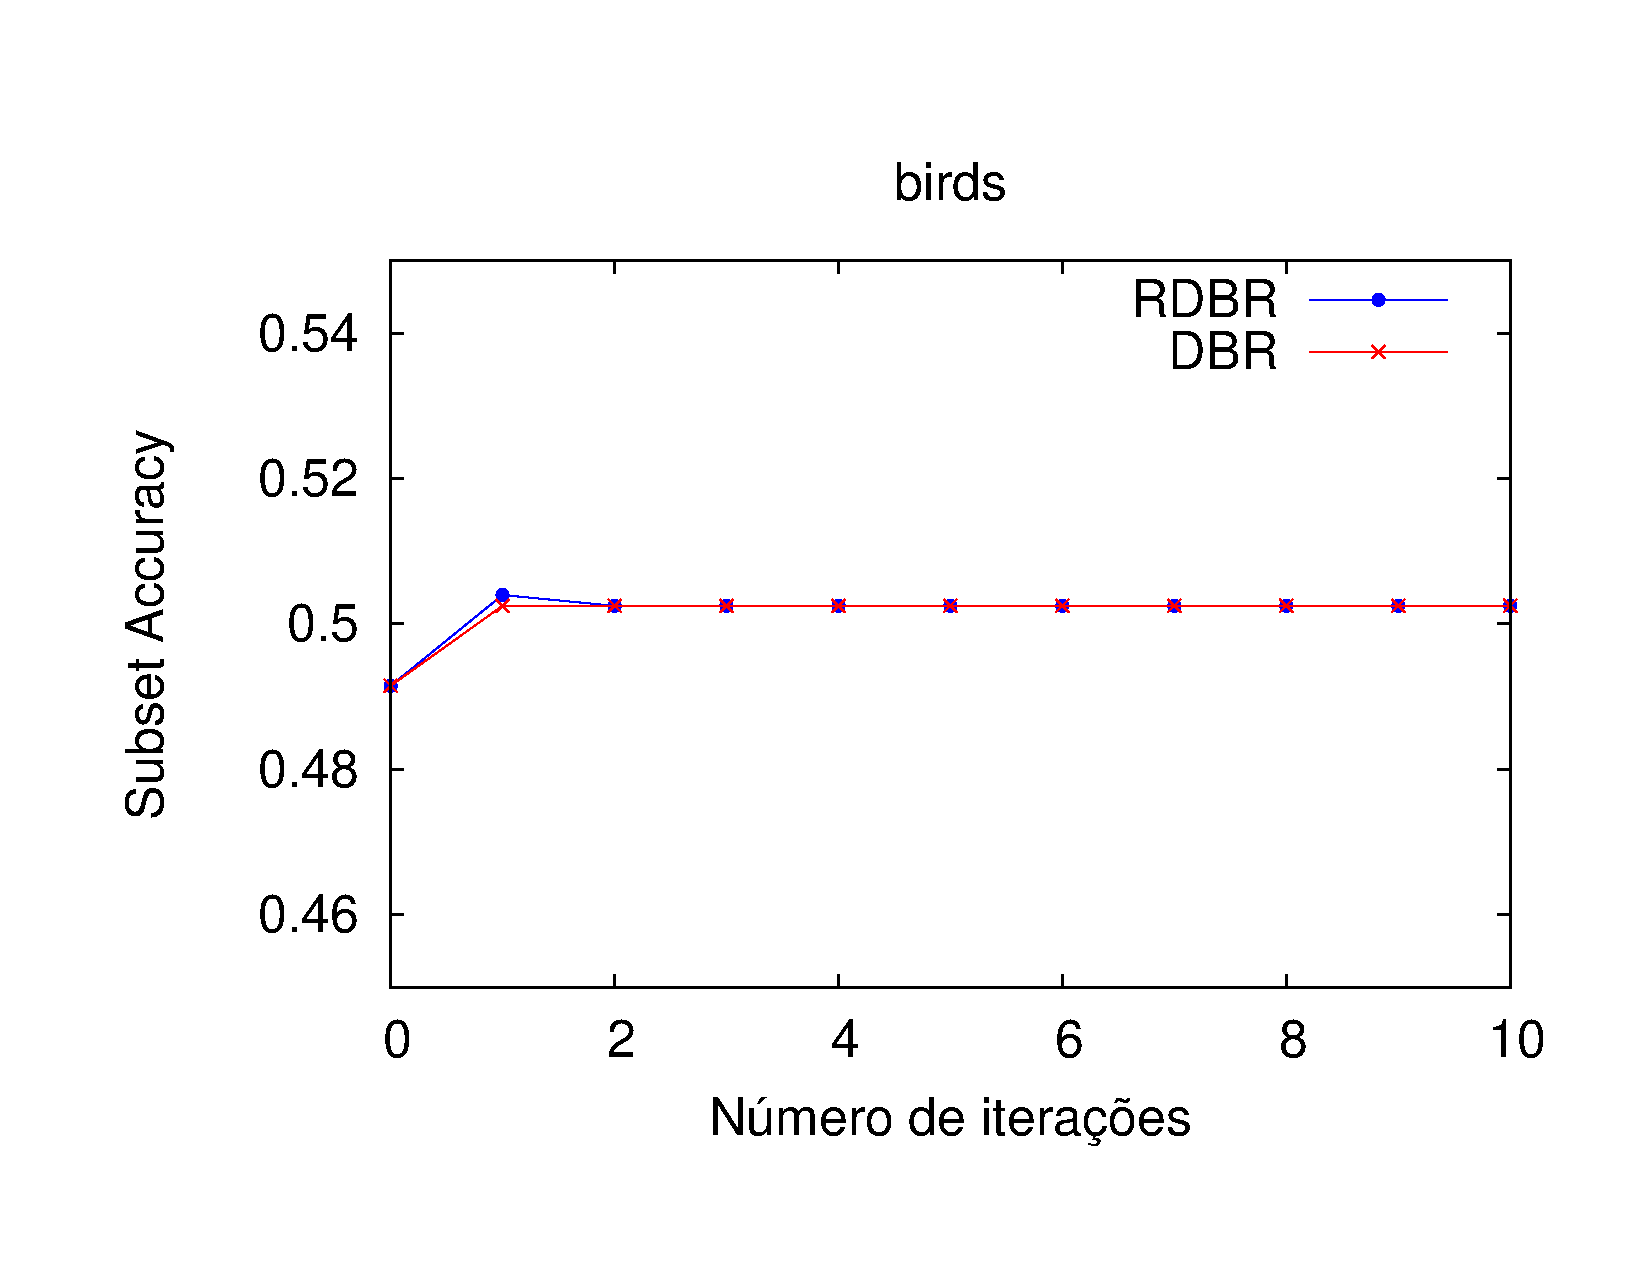
\includegraphics[angle=-90, width=1\linewidth]{plots/birds.pdf}
  \caption{Birds}
  \label{fig:subbirds}
\end{subfigure}%
\begin{subfigure}{.5\textwidth}
  \centering
  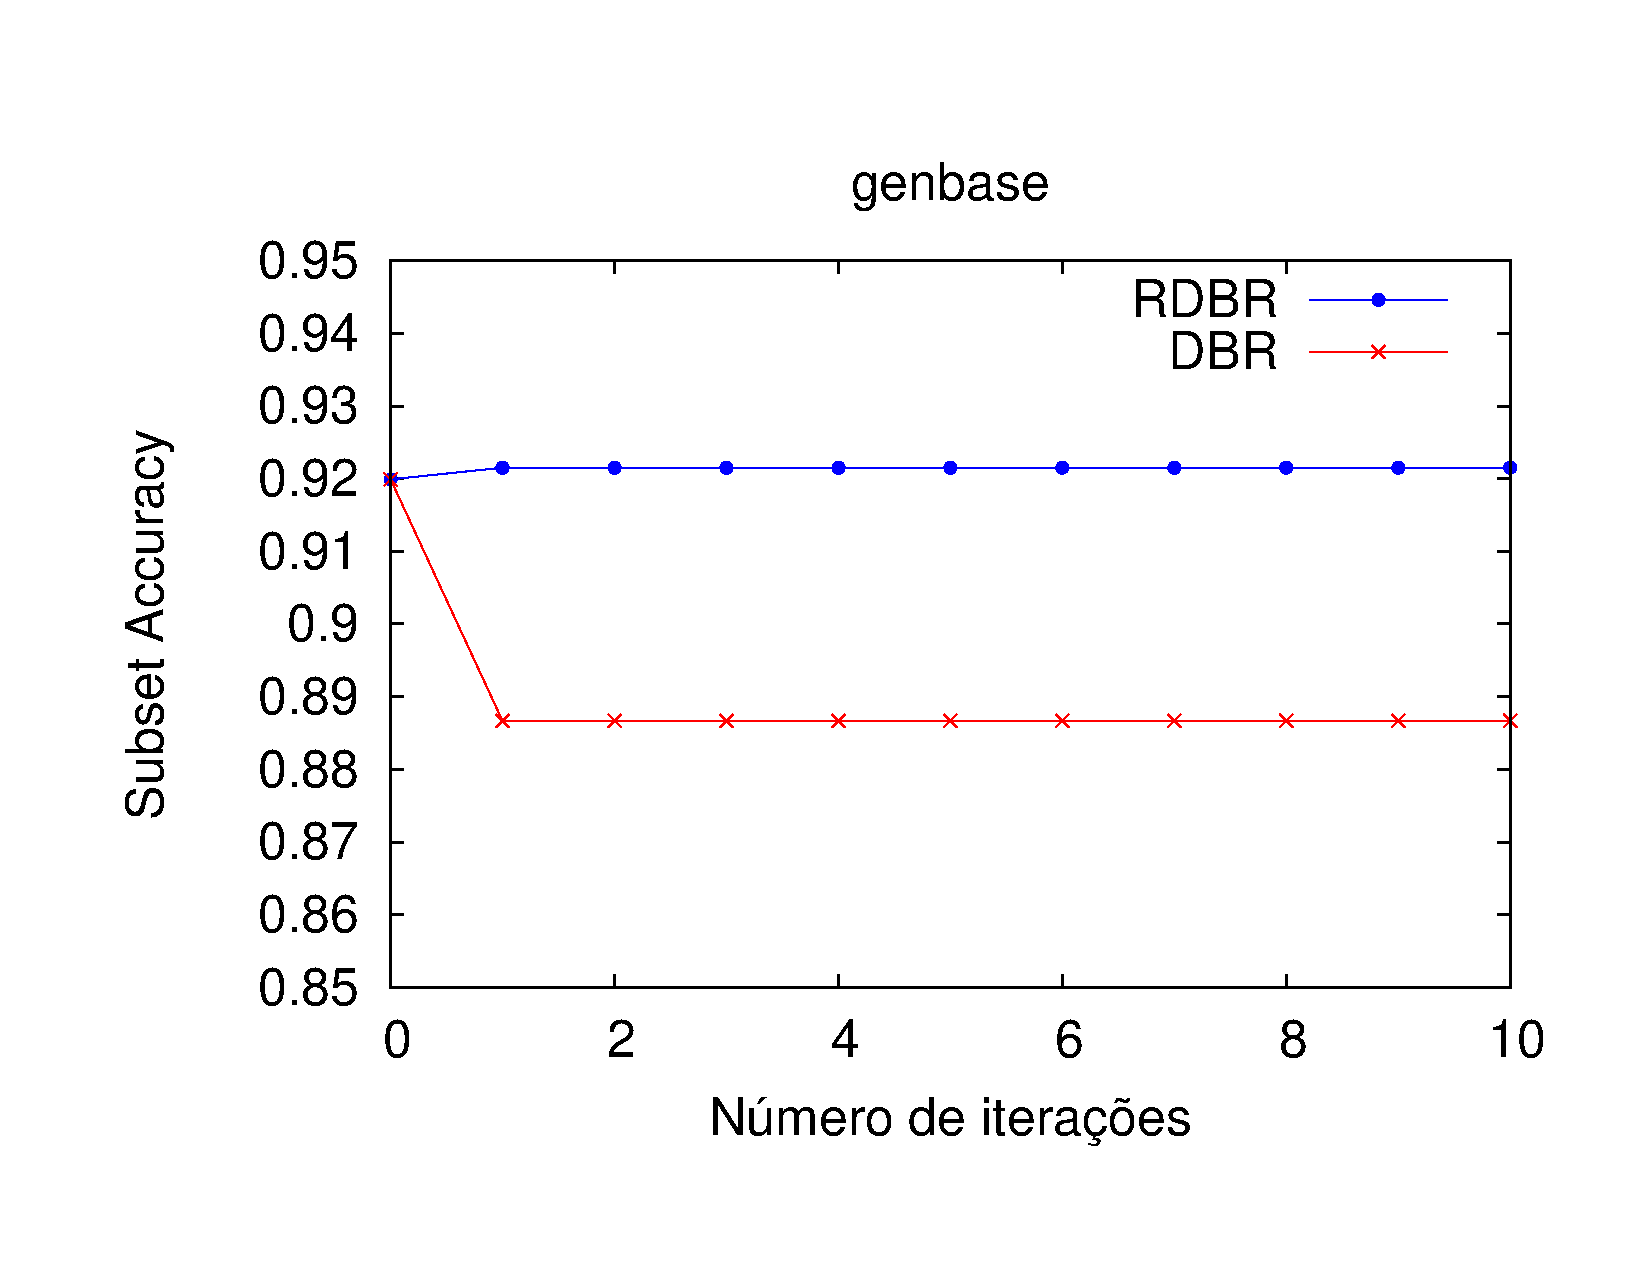
\includegraphics[angle=-90, width=1\linewidth]{plots/genbase.pdf}
  \caption{Genbase}
  \label{fig:subgenbase}
\end{subfigure}

\caption{Gráficos de análise de desempenho do \MRLMa~nos dois experimentos em que
o \MRLMa~não melhorou na sua segunda iteração.}
\label{fig:mrlmgraph2}
\end{figure}



É importante analisar o quanto o método aumenta o tamanho da base de dados uma vez que isso acarreta no aumento
do tempo de execução do algoritmo. Seja $r$ o número de rótulos, $n$ o número de instâncias de treino
e $m$ o número de atributos da base original, na fase de treinamento do \MRLMa, o número de base de dados utilizadas são
$2r$, cada uma contendo $n$ instâncias. Em metade delas, as instâncias contidas tem $m$ atributos e na outra metade $m+r$ atributos.
Já na fase de predição do algoritmo, no pior caso, o algoritmo usa $(k+1)r$ bases de dados de $n$ instâncias onde na primeira base, o
número de atributos é igual a $m$ e nas restantes é igual $m+r$. Vale ressaltar que nem todas essas bases de dados precisam ser
armazenados explicitamente na mémoria em espaços diferentes, algumas podem são reutilizadas no processo de predição.

% Em relação a complexidade algorítma do \MRLMa, ela pode ser
% aproximada pelo número de atributos destinados ao classificador base, uma vez que é um método de transformação
% e a maior parte do custo computacional se encontra no classificador base.
% A complexidade 




\chapter{Avaliação e Análise Experimental}
Neste capítulo é descrito as bases de dados multirrótulo usadas nos experimentos, as medidas de avaliação escolhidas e a escolha
dos parâmetros dos classificadores. 
A comparação e estudo dos métodos é feita considerando o custo computacional e a qualidade de predição.
A qualidade de predição é estimada pelo método de avaliação por validação cruzada \ref{sec:modelav} com 10 grupos
(\textit{10-fold cross-validation}) sobre \Nbases~bases de dados, todas apresentadas e descritas na subseção \ref{sec:datas}.

Para quantificar a qualidade de predição, 3 métricas foram utilizadas.
As métricas escolhidas, bem como o motivo das escolhas,
são listadas:
\begin{itemize}
 \item Subset Accuracy, pois é mostrado que captura bem a correlação entre rótulos;
 \item Hamming Loss, pois é bem mais sensível que o Subset Accuracy;
 \item Example Based Accuracy, é o meio termo entre o Hamming Loss e o Subset Accuracy.
%  \item Tempo computacional, pois é @@@ etc...
\end{itemize}

As fórmulas para o cálculo de cada uma das métricas são apresentadas na seção \ref{sec:metrics}.
É interessante mostrar os resultados experimentais usando diferentes métricas, pois cada uma captura
um aspecto diferente da classificação. 

A análise experimental dos métodos se encontram divididos em dois estudos. O primeiro estudo consiste em
comparar os métodos quando todos usam o mesmo classificador base e o segundo em comparar cada combinação de um
modelo de classificação multirrótulo com uma configuração de parâmetros definida. 
O primeiro estudo, que chamaremos de Estudo Específico, tem por objetivo analisar se cada método multirrótulo apresentada desempenhos diferentes para
diferentes classificadores, ou seja, se o \textit{ranking} é alterado ao alterar o classificador base.
O segundo estudo, que chamaremos de Estudo Geral,
tem por objetivo analisar os métodos de uma forma geral,
desconhecendo o classificador base que melhor se adapta a cada base, a priori.
Nesse estudo, cada combinação de modelo multirrótulo com um classificador base é considerado
um novo método multirrótulo.

Num total, foram utilizados \Nml~modelos de classificação multirrótulos: BR, DBR, RDBR, CC, ECC e MCC.
Para cada um deles utilizou-se os seguintes classificadores base KNN, SVM, \jqo e Regressão Logística.
Implementações públicas dos classificadores na biblioteca \textit{Weka} \cite{weka} foram usados para este trabalho.
A seguir a descrição de cada um deles.

\begin{itemize}
 \item \textbf{KNN}: O KNN é uma das técnicas do aprendizado supervisionado mais conhecida. 
 O KNN funciona da seguinte forma: Uma instância de características $x',x'\in X$
 e de classe desconhecida é classificado baseado
 nas classes dos $K$ vizinhos mais próximos, onde mais próximo entende-se por aquela instância
 $(x,y)$, para $x \in X$ e $y \in Y$,
 cuja distância euclidiana entre os vetores reais $x$ e $x'$ é mínima. 
 A classe predominante dos $K$ vizinhos mais próximos será a classe atribuída para $x'$ \cite{topalgos2008}.
 
 \item \textbf{SVM}: 
 Em um problema de classificação binária, o objetivo do SVM é encontrar o melhor hiperplano, 
 definida pela função de hiperplano $h(x)=0$ para $x \in X$,
 que separa as duas classes na base de treino.
 O ``melhor'' hiperplano é definido como aquele que simultaneamente minimiza
 o erro de classificação e maximiza a distância do hiperplano à instância mais próxima dele \cite{topalgos2008}. 
 
 
 \item \textbf{\jqo}: 
 O \jqo~é um algoritmo para contruir uma árvore de decisão.
 Segundo \cite{peng2009implementation} uma árvore de decisão é uma
 árvore cujos nós folhas representam decisões e os nós não-folhas representam
 uma escolha entre alternativas. Cada nó não-folha é associado a um atributo da base e
 cada ligação desse nó a seus nós filhos está associado a um valor possível desse atributo.
 Cada nó folha é associado a uma classe.
 Quando uma instância de teste é submetida ao classificador, o algoritmo começa nó raiz e caminha
 em direção ao nó filho cuja ligação está associado ao mesmo valor do atributo que a instância de teste tem.
 O algoritmo continua nesse mesmo processo, caminhando sobre os nós e ligações até chegar a um nó folha, onde então
 a instância de teste é classificado com a classe associada ao nó folha.
 A quantidade de nós e as associações dos nós as seus respectivos atributos,valores de atributos ou classes
 são feitas pelo algoritmo
 de construção da árvore, que nesse trabalho utilizamos o \jqo.

 \item \textbf{Regressão Logística}
 Segundo \cite{james2013introduction} o classificador baseado na Regressão Logística 
 é um modelo probabilístico da estatística. Num problema de classificação binária,
 esse classificador usa um modelo de regressão não-linear
 para calcular a probabilidade de um instância qualquer pertencer a classe positiva.
 O modelo de regressão não-linear usado é a função logística, 
 \begin{equation} \label{eq:RL}
  p(\yy=1|\xx) = \frac{e^{\ww \cdot \xx}}{1+e^{\ww \cdot \xx}}
 \end{equation}
onde $\xx$ é o vetor de características, $\yy$ é a classe positiva e $\ww$ é um vetor de coeficientes de mesma dimensão
que $\xx$ o qual é estimado durante a fase de treinamento do algoritmo pela máxima verossimilhança \cite{james2013introduction}.
Pela equação \ref{eq:RL} podemos calcular a probabilidade de uma instância de características $\xx$ pertencer a classe $\yy$.
 
 
\end{itemize}


% Para o melhor entendimento, neste capítulo um método multirrótulo é definido como sendo a combinação
% de um modelo de classificação multirrótulo com uma configuração de parâmetros pré-definida. Assim, por exemplo,
% o classificador BR com KNN é considerado um método diferente do classificador BR com SVM.
% Isso, por um lado é bom
% pois testa o desempenho dos classificadores multirrótulo quando não é gasto tempo computacional para ajustar parâmetros.
% Por outro lado é ruim uma vez que considera os mesmos modelos de classificação como sendo completamente diferentes.
% Dessa forma, foram considerados 24 métodos multirrótulos e comparados entre si de forma experimental.


\section{Base de dados}
\label{sec:datas}
As bases de dados são apresentadas na tabela \ref{tab:datas}.
Sete das oito bases de dados utilizadas nos experimentos foram obtidas do repositório público
de endereço virtual http://mulan.sourceforge.net/datasets.html.
A única base de dados não obtida pelo repositório público acima é a nomeada Motorpump, que é uma
base de dados privada \cite{mendel2008}.



% Yeast:
%  Emotions: 
%  Medical:
%  Eron: Pertencente ao domínio de bases de dados do tipo texto a eron possui um
% número de 1702 instanciam relacionadas com 53 rótulos e 1001 atributos discretos.
% 
% 
% 
% \begin{itemize}
% \item \bf{Birds}: ??
% 
% \item \bf{Emotions}: A base de dados emoctions (Wieczorkowska, Synak, and Rás 2006 apud
% Santos, 2012 apud SÁ, 2008) está relacionada com a classificação de músicas de
% acordo com as emoções, esta base possui um número de 593 instancias associadas a
% um subconjunto de 6 rótulos. Cada instância possui 72 atributos numéricos e 0
% atributos discretos.
% \item \bf{Enron}: ??
% 
% \item \bf{Genbase}: ??
% 
% \item \bf{Medical}:  A base de dados Medical é composta de documentos com um resumo de
% texto livre de histórias de sintomas e prognóstico que são usados para prever códigos
% seguros e está disponível no site
% http://www.computationalmedicine.org/challenge/index.php. Esta base de dados
% contém 978 instâncias, descritas por 1449 atributos discretos, com possibilidade de
% associação a 45 rótulos (classes).
% 
% \item \bf{Motorpump}: ??
% 
% \item \bf{Scene}: ??
% 
% \item \bf{Yeast}: a base de dados biológicos yeast (Clare and king 2001 apud SÁ, 2008) esta
% relacionada a classificação de funções de proteínas. Está base contém microvetores de
% expressões e perfis filogenéticos de 2417 instancias (exemplos). Onde cada instancia
% está associada a um subconjunto de 14 categorias (rótulos) possíveis do nível mais
% acima do catálogo funcional (FunCat). Cada instância apresenta 103 atributos
% numéricos (NUM) e 0 atributos discretos (DIS).
% 
% \end{itemize}

\begin{table}[h]
\begin{tabular}{|c|ccccccc|}
\hline
% \textbf{}         & \textbf{}        & \textbf{}         & \multicolumn{2}{c}{\textbf{ATRIBUTOS}} & \textbf{}        & \textbf{}              & \textbf{}          \\
\textbf{BASE}      & \textbf{DOM} & \textbf{EXEMPLOS} & \textbf{DIS} & \textbf{NUM} & \textbf{RÓTULOS} & \textbf{CARD} & \textbf{DENS} \\ \hline
\textbf{Birds}     & Audio            & 645               & 2                 & 258                & 19               & 1.014                  & 0.053              \\
\textbf{Emotions}  & Música           & 593               & 0                 & 72                 & 6                & 1.869                  & 0.311              \\
\textbf{Enron}     & Texto            & 1702              & 1001              & 0                  & 53               & 3.378                  & 0.064              \\
\textbf{Genbase}   & Biologia         & 662               & 1186              & 0                  & 27               & 1.252                  & 0.046              \\
\textbf{Medical}   & Texto            & 978               & 1449              & 0                  & 45               & 1.245                  & 0.028              \\
\textbf{Motorpump} & ??               & 1372              & 0                 & 40                 & 9                & 2.249                  & 0.250              \\
\textbf{Scene}     & Imagem           & 2407              & 0                 & 294                & 6                & 1.074                  & 0.179              \\
\textbf{Yeast}     & Biologia         & 2417              & 0                 & 103                & 14               & 4.237                  & 0.303              \\  \hline

\end{tabular}
\caption{Resumo das bases de dados multirrótulos}
\label{tab:datas}
\end{table}

A tabela \ref{tab:datas} apresenta algumas estatísticas das bases de dados adquiridas.
Nela são apresentadas as seguintes informações de cada base de dados:
\begin{itemize}
  \item \textbf{DOM}: Domínio pertencente;
  \item \textbf{DIS}: número de atributos discretos;
  \item \textbf{NUM}: número de atributos numéricos;
  \item \textbf{CARD}: cardinalidade de rótulos na base de dados;
  \item \textbf{DENS}: densidade de rótulos na base de dados.
\end{itemize}


% \section{Método de Comparação}
% \label{sec:methodcomp}


% 
% Este capítulo se encontra dividido em duas seções, na primeira foram analisados os
% resultados dos métodos de transformação para cada classificador base.
% Já na segunda seção cada combinação de método multirrótulo com classificador base foi considerado
% um método de transformação e seus resultados são comparados entre si juntamente com os métodos multirrótulos
% de adaptação.


\section{Resultados Experimentais}
\label{sec:exps}
Nesta seção é feita uma análise do desempenho dos métodos multirrótulos em cada uma das bases de dados
em diferentes métricas.
Essa seção é dividida em 2 subseções, um para o Estudo específico citado e
outro para o Estudo Geral, ambos definidos no ínicio do capítulo.

No Estudo Específico os métodos tiveram seus classificadores bases fixados.
A razão disso vem do fato de que queremos comparar os métodos multirrótulos entre si,
e não os seus classificadores bases.
Ao fixarmos o classificador base, 
o desempenho irá depender apenas do modelo de classificação multirrótulo
de cada um.
Em cada subseção e para cada métrica escolhida é apresentado uma tabela
contendo os valores da métrica para cada um dos métodos multirrótulo e
o ranking dos métodos multirrótulos.



\subsection{Estudo Específico}
% \begin{table}[h]
\begin{tabular}{lllllll}
\hline
\textbf{Dataset}    & \textbf{BR} & \textbf{CC} & \textbf{DBR} & \textbf{ECC} & \textbf{MCC} & \textbf{RDBR} \\ \hline
\textbf{Birds}      & 0.5084(3)   & 0.5007(5)   & 0.5116(1)    & 0.4991(6)    & 0.5023(4)    & 0.5115(2)     \\
\textbf{Emotions}   & 0.3101(5)   & 0.3406(1)   & 0.3119(4)    & 0.3(6)       & 0.3287(3)    & 0.3355(2)     \\
\textbf{Enron}      & 0.0717(5)   & 0.0899(3)   & 0.1005(2)    & 0.077(4)     & 0.0664(6)    & 0.1022(1)     \\
\textbf{Genbase}    & 0.9351(4)   & 0.9411(1)   & 0.9396(2)    & 0.0(6)       & 0.9336(5)    & 0.9381(3)     \\
\textbf{Medical}    & 0.4519(6)   & 0.503(2)    & 0.5(3)       & 0.4796(5)    & 0.4847(4)    & 0.5133(1)     \\
\textbf{Motorpump}  & 0.2857(1)   & 0.2799(4)   & 0.266(6)     & 0.2821(2)    & 0.2806(3)    & 0.2791(5)     \\
\textbf{Scene}      & 0.6452(6)   & 0.668(3)    & 0.6498(5)    & 0.661(4)     & 0.6788(2)    & 0.7009(1)     \\
\textbf{Yeast}      & 0.2209(6)   & 0.2454(3)   & 0.2226(5)    & 0.2301(4)    & 0.2615(1)    & 0.247(2)      \\ \hline
\textbf{Rank médio} & 4.5         & 2.75        & 3.5          & 4.625        & 3.5          & 2.125         \\ \hline
\end{tabular}
\caption{\legendaTab{Subset Accuracy}{KNN}}
\label{tab:SAknn}
\end{table}
% \begin{table}[h]
\begin{tabular}{lllllll}
\hline
\textbf{Dataset}    & \textbf{BR} & \textbf{CC} & \textbf{DBR} & \textbf{ECC} & \textbf{MCC} & \textbf{RDBR} \\ \hline
\textbf{Birds}      & 0.0453(1)   & 0.0489(6)   & 0.0476(5)    & 0.0463(2)    & 0.0474(4)    & 0.0469(3)     \\
\textbf{Emotions}   & 0.1937(1)   & 0.2041(3)   & 0.2159(6)    & 0.1973(2)    & 0.2063(4)    & 0.2068(5)     \\
\textbf{Enron}      & 0.0581(1.5) & 0.059(3.5)  & 0.0606(5)    & 0.0581(1.5)  & 0.059(3.5)   & 0.0607(6)     \\
\textbf{Genbase}    & 0.0031(1)   & 0.0033(2)   & 0.0059(5)    & 1.0(6)       & 0.0038(4)    & 0.0034(3)     \\
\textbf{Medical}    & 0.0175(3.5) & 0.0165(1)   & 0.0188(5)    & 0.0171(2)    & 0.0175(3.5)  & 0.0189(6)     \\
\textbf{Motorpump}  & 0.1618(2)   & 0.1697(3)   & 0.1864(6)    & 0.161(1)     & 0.1714(5)    & 0.171(4)      \\
\textbf{Scene}      & 0.0925(2)   & 0.1003(5)   & 0.1065(6)    & 0.0931(3)    & 0.0965(4)    & 0.0906(1)     \\
\textbf{Yeast}      & 0.1981(2)   & 0.2159(6)   & 0.2109(5)    & 0.195(1)     & 0.2054(4)    & 0.2031(3)     \\ \hline
\textbf{Rank médio} & 1.75        & 3.6875      & 5.375        & 2.3125       & 4            & 3.875         \\ \hline
\end{tabular}
\caption{\legendaTab{Hamming Loss}{KNN}}
\label{tab:HLknn}
\end{table}
% \begin{table}[h]
\begin{tabular}{lllllll}
\hline
\textbf{Dataset}    & \textbf{BR} & \textbf{CC} & \textbf{DBR} & \textbf{ECC} & \textbf{MCC} & \textbf{RDBR} \\ \hline
\textbf{Birds}      & 0.58(1)     & 0.5689(2)   & 0.5656(3)    & 0.5555(6)    & 0.5648(5)    & 0.5651(4)     \\
\textbf{Emotions}   & 0.5515(5)   & 0.5765(1)   & 0.5737(2)    & 0.545(6)     & 0.5604(4)    & 0.5691(3)     \\
\textbf{Enron}      & 0.2344(4)   & 0.2456(3)   & 0.264(2)     & 0.2198(5)    & 0.2085(6)    & 0.265(1)      \\
\textbf{Genbase}    & 0.9601(4)   & 0.9639(1)   & 0.9628(2)    & 0.0(6)       & 0.96(5)      & 0.9621(3)     \\
\textbf{Medical}    & 0.5147(6)   & 0.5724(3)   & 0.5966(1)    & 0.5455(5)    & 0.5476(4)    & 0.5857(2)     \\
\textbf{Motorpump}  & 0.5452(1)   & 0.5359(2)   & 0.5123(6)    & 0.5346(3)    & 0.5289(4)    & 0.5245(5)     \\
\textbf{Scene}      & 0.6742(6)   & 0.6987(4)   & 0.7123(2)    & 0.692(5)     & 0.7089(3)    & 0.7322(1)     \\
\textbf{Yeast}      & 0.524(4)    & 0.52(6)     & 0.5238(5)    & 0.5361(2)    & 0.5368(1)    & 0.5343(3)     \\ \hline
\textbf{Rank médio} & 3.875       & 2.75        & 2.875        & 4.75         & 4            & 2.75          \\ \hline
\end{tabular}
\caption{\legendaTab{\EBA}{KNN}}
\label{tab:EBAknn}
\end{table}
% 
% \begin{table}[h]
\begin{tabular}{lllllll}
\hline
\textbf{Dataset} & \textbf{BR} & \textbf{CC} & \textbf{DBR} & \textbf{ECC} & \textbf{MCC} & \textbf{RDBR} \\ \hline
\textbf{Birds}           & 0.4775(2)   & 0.4496(6)   & 0.4528(4)    & 0.4604(3)    & 0.4822(1)    & 0.4527(5)     \\
\textbf{Emotions}        & 0.2917(6)   & 0.3051(5)   & 0.3086(4)    & 0.3356(2)    & 0.3255(3)    & 0.3558(1)     \\
\textbf{Enron}           & 0.0741(6)   & 0.1052(4)   & 0.094(5)     & 0.1334(1)    & 0.1087(2)    & 0.1075(3)     \\
\textbf{Genbase}         & 0.9033(5)   & 0.9154(1)   & 0.9123(3)    & 0.8836(6)    & 0.9047(4)    & 0.9139(2)     \\
\textbf{Medical}         & 0.5931(6)   & 0.6228(4.5) & 0.6228(4.5)  & 0.6483(1)    & 0.6361(3)    & 0.6443(2)     \\
\textbf{Motorpump}       & 0.2186(6)   & 0.2755(3)   & 0.2558(5)    & 0.293(1)     & 0.2748(4)    & 0.2763(2)     \\
\textbf{Scene}           & 0.5322(6)   & 0.6394(3)   & 0.5422(5)    & 0.6572(1)    & 0.6548(2)    & 0.614(4)      \\
\textbf{Yeast}           & 0.1489(6)   & 0.1965(3)   & 0.1535(5)    & 0.2006(2)    & 0.2193(1)    & 0.1845(4)     \\ \hline
\textbf{Rank médio}      & 5.375       & 3.6875      & 4.4375       & 2.125        & 2.5          & 2.875         \\ \hline
\end{tabular}
\caption{\legendaTab{Subset Accuracy}{SVM}}
\label{tab:SAsvm}
\end{table}
% \begin{table}[h]
\begin{tabular}{lllllll}
\hline
\textbf{Dataset}    & \textbf{BR} & \textbf{CC} & \textbf{DBR} & \textbf{ECC} & \textbf{MCC} & \textbf{RDBR} \\ \hline
\textbf{Birds}      & 0.0596(2)   & 0.0651(4)   & 0.0662(6)    & 0.0567(1)    & 0.0624(3)    & 0.066(5)      \\
\textbf{Emotions}   & 0.1917(2)   & 0.2134(5)   & 0.2156(6)    & 0.1847(1)    & 0.2108(4)    & 0.1929(3)     \\
\textbf{Enron}      & 0.0799(6)   & 0.0744(3.5) & 0.0744(3.5)  & 0.0529(1)    & 0.0726(2)    & 0.0762(5)     \\
\textbf{Genbase}    & 0.0041(5)   & 0.0036(2)   & 0.0035(1)    & 0.0051(6)    & 0.004(4)     & 0.0037(3)     \\
\textbf{Medical}    & 0.0127(6)   & 0.0126(4.5) & 0.0125(2.5)  & 0.0112(1)    & 0.0125(2.5)  & 0.0126(4.5)   \\
\textbf{Motorpump}  & 0.1657(2)   & 0.167(4)    & 0.1701(6)    & 0.154(1)     & 0.1685(5)    & 0.1659(3)     \\
\textbf{Scene}      & 0.1066(3)   & 0.1067(4)   & 0.2094(6)    & 0.0903(1)    & 0.1029(2)    & 0.1167(5)     \\
\textbf{Yeast}      & 0.2001(1)   & 0.2246(6)   & 0.221(5)     & 0.2027(2)    & 0.2108(4)    & 0.2103(3)     \\ \hline
\textbf{Rank médio} & 3.375       & 4.125       & 4.5          & 1.75         & 3.3125       & 3.9375        \\ \hline
\end{tabular}
\caption{\legendaTab{Hamming Loss}{SVM}}
\label{tab:HLsvm}
\end{table}
% \begin{table}[\tabmode]
\begin{tabular}{lllllll}
\hline
\textbf{Dataset}    & \textbf{BR} & \textbf{CC} & \textbf{DBR} & \textbf{ECC} & \textbf{MCC} & \textbf{RDBR} \\ \hline
\textbf{Birds}      & 0.6068(1)   & 0.586(4)    & 0.5786(6)    & 0.5975(3)    & 0.6041(2)    & 0.5828(5)     \\
\textbf{Emotions}   & 0.5345(6)   & 0.5434(5)   & 0.5842(2)    & 0.5781(3)    & 0.5541(4)    & 0.6018(1)     \\
\textbf{Enron}      & 0.3503(6)   & 0.3728(3)   & 0.3661(5)    & 0.4331(1)    & 0.382(2)     & 0.3688(4)     \\
\textbf{Genbase}    & 0.9552(5)   & 0.9608(1)   & 0.9603(2)    & 0.9444(6)    & 0.9555(4)    & 0.9597(3)     \\
\textbf{Medical}    & 0.6983(6)   & 0.713(4)    & 0.714(3)     & 0.7226(2)    & 0.7128(5)    & 0.727(1)      \\
\textbf{Motorpump}  & 0.465(6)    & 0.5275(5)   & 0.5488(2)    & 0.5535(1)    & 0.5286(4)    & 0.5398(3)     \\
\textbf{Scene}      & 0.6065(6)   & 0.6916(3)   & 0.6233(5)    & 0.7036(1)    & 0.7018(2)    & 0.6604(4)     \\
\textbf{Yeast}      & 0.5064(4)   & 0.4921(6)   & 0.4949(5)    & 0.5243(2)    & 0.5258(1)    & 0.5142(3)     \\ \hline
\textbf{Rank médio} & 5           & 3.875       & 3.75         & 2.375        & 3            & 3             \\ \hline
\end{tabular}
\caption{\legendaTab{\EBA}{SVM}}
\label{tab:EBAsvm}
\end{table}
% 
% \begin{table}[h]
\begin{tabular}{lllllll}
\hline
\textbf{Dataset}    & \textbf{BR} & \textbf{CC} & \textbf{DBR} & \textbf{ECC} & \textbf{MCC} & \textbf{RDBR} \\ \hline
\textbf{Birds}      & 0.4683(6)   & 0.4791(4)   & 0.49(2.5)    & 0.5318(1)    & 0.4775(5)    & 0.49(2.5)     \\
\textbf{Emotions}   & 0.1637(6)   & 0.1888(4)   & 0.1822(5)    & 0.3002(1)    & 0.2328(2)    & 0.2244(3)     \\
\textbf{Enron}      & 0.1034(5)   & 0.1257(2)   & 0.0975(6)    & 0.1381(1)    & 0.114(3)     & 0.1116(4)     \\
\textbf{Genbase}    & 0.9714(2.5) & 0.9699(5)   & 0.9714(2.5)  & 0.9623(6)    & 0.9714(2.5)  & 0.9714(2.5)   \\
\textbf{Medical}    & 0.6718(6)   & 0.6902(4)   & 0.6974(2)    & 0.6739(5)    & 0.6932(3)    & 0.7035(1)     \\
\textbf{Motorpump}  & 0.2274(6)   & 0.2536(3)   & 0.2376(5)    & 0.3185(1)    & 0.2442(4)    & 0.2573(2)     \\
\textbf{Scene}      & 0.4408(5)   & 0.5692(2)   & 0.4366(6)    & 0.5962(1)    & 0.5501(3)    & 0.543(4)      \\
\textbf{Yeast}      & 0.0658(6)   & 0.1448(2)   & 0.0666(5)    & 0.1684(1)    & 0.1303(3)    & 0.1212(4)     \\ \hline
\textbf{Rank médio} & 5.3125      & 3.25        & 4.25         & 2.125        & 3.1875       & 2.875         \\ \hline
\end{tabular}
\caption{\legendaTab{Subset Accuracy}{\jqo}}
\label{tab:SAj48}
\end{table}
% \begin{table}[h]
\begin{tabular}{lllllll}
\hline
\textbf{Dataset}    & \textbf{BR} & \textbf{CC} & \textbf{DBR} & \textbf{ECC} & \textbf{MCC} & \textbf{RDBR} \\ \hline
\textbf{Birds}      & 0.0517(5)   & 0.0501(2)   & 0.051(3.5)   & 0.0415(1)    & 0.052(6)     & 0.051(3.5)    \\
\textbf{Emotions}   & 0.2529(2)   & 0.2693(5)   & 0.2729(6)    & 0.1945(1)    & 0.2575(3)    & 0.2645(4)     \\
\textbf{Enron}      & 0.0509(2)   & 0.054(5)    & 0.0559(6)    & 0.049(1)     & 0.0532(3)    & 0.0537(4)     \\
\textbf{Genbase}    & 0.0012(2.5) & 0.0013(5)   & 0.0012(2.5)  & 0.0016(6)    & 0.0012(2.5)  & 0.0012(2.5)   \\
\textbf{Medical}    & 0.01(5)     & 0.0097(3.5) & 0.0093(1)    & 0.0101(6)    & 0.0097(3.5)  & 0.0095(2)     \\
\textbf{Motorpump}  & 0.1753(3)   & 0.174(2)    & 0.1791(6)    & 0.1398(1)    & 0.1769(4)    & 0.1782(5)     \\
\textbf{Scene}      & 0.1307(2)   & 0.1334(3)   & 0.1779(6)    & 0.0941(1)    & 0.1378(4)    & 0.1449(5)     \\
\textbf{Yeast}      & 0.2489(2)   & 0.268(4)    & 0.2829(6)    & 0.2046(1)    & 0.2702(5)    & 0.2637(3)     \\ \hline
\textbf{Rank médio} & 2.9375      & 3.6875      & 4.625        & 2.25         & 3.875        & 3.625         \\ \hline
\end{tabular}
\caption{\legendaTab{Hamming Loss}{\jqo}}
\label{tab:HLj48}
\end{table}
% \begin{table}[\tabmode]
\begin{tabular}{lllllll}
\hline
\textbf{Dataset}    & \textbf{BR} & \textbf{CC} & \textbf{DBR} & \textbf{ECC} & \textbf{MCC} & \textbf{RDBR} \\ \hline
\textbf{Birds}      & 0.5628(6)   & 0.5706(4)   & 0.5764(3)    & 0.5935(1)    & 0.5629(5)    & 0.5777(2)     \\
\textbf{Emotions}   & 0.4447(4)   & 0.4405(5)   & 0.4176(6)    & 0.5238(1)    & 0.469(2)     & 0.4631(3)     \\
\textbf{Enron}      & 0.4131(4)   & 0.4115(5)   & 0.4141(3)    & 0.44(1)      & 0.3989(6)    & 0.4163(2)     \\
\textbf{Genbase}    & 0.9854(2.5) & 0.9847(5)   & 0.9854(2.5)  & 0.9779(6)    & 0.9854(2.5)  & 0.9854(2.5)   \\
\textbf{Medical}    & 0.7585(5)   & 0.7707(4)   & 0.7822(2)    & 0.7573(6)    & 0.7732(3)    & 0.7845(1)     \\
\textbf{Motorpump}  & 0.5252(6)   & 0.549(2)    & 0.5347(5)    & 0.6046(1)    & 0.5393(4)    & 0.5444(3)     \\
\textbf{Scene}      & 0.54(5)     & 0.6205(2)   & 0.5336(6)    & 0.6276(1)    & 0.6011(3)    & 0.5843(4)     \\
\textbf{Yeast}      & 0.4357(3)   & 0.4252(4)   & 0.4171(6)    & 0.4932(1)    & 0.4196(5)    & 0.4451(2)     \\ \hline
\textbf{Rank médio} & 4.4375      & 3.875       & 4.1875       & 2.25         & 3.8125       & 2.4375        \\ \hline
\end{tabular}
\caption{\legendaTab{\EBA}{\jqo}}
\label{tab:EBAj48}
\end{table}
% 
% \begin{table}[h]
\begin{tabular}{lllllll}
\hline
\textbf{Subset Accuracy} & \textbf{BR} & \textbf{CC} & \textbf{DBR} & \textbf{ECC} & \textbf{MCC} & \textbf{RDBR} \\ \hline
\textbf{Birds}           & 0.4403(6)   & 0.4512(2)   & 0.4434(5)    & 0.4836(1)    & 0.448(3.5)   & 0.448(3.5)    \\
\textbf{Emotions}        & 0.2343(5)   & 0.268(1)    & 0.2073(6)    & 0.2561(2)    & 0.2411(4)    & 0.2427(3)     \\
\textbf{Enron}           & 0.1093(3)   & 0.1134(2)   & 0.1017(6)    & 0.1257(1)    & 0.1081(4)    & 0.107(5)      \\
\textbf{Genbase}         & 0.9562(4)   & 0.9532(5)   & 0.9577(2)    & 0.7901(6)    & 0.9577(2)    & 0.9577(2)     \\
\textbf{Medical}         & 0.4499(6)   & 0.4653(5)   & 0.4684(4)    & 0.5297(1)    & 0.4745(3)    & 0.4827(2)     \\
\textbf{Motorpump}       & 0.2857(6)   & 0.3003(3)   & 0.2944(5)    & 0.3039(1)    & 0.2995(4)    & 0.301(2)      \\
\textbf{Scene}           & 0.4989(5)   & 0.6003(2)   & 0.4944(6)    & 0.5941(3)    & 0.6061(1)    & 0.5845(4)     \\
\textbf{Yeast}           & 0.1369(6)   & 0.1841(2)   & 0.1386(5)    & 0.1709(3)    & 0.1907(1)    & 0.168(4)      \\ \hline
\textbf{Rank médio}      & 5.125       & 2.75        & 4.875        & 2.25         & 2.8125       & 3.1875        \\ \hline
\end{tabular}
\caption{\legendaTab{Subset Accuracy}{Regressão Logística}}
\label{tab:SAlogi}
\end{table}
% \begin{table}[h]
\begin{tabular}{lllllll}
\hline
\textbf{Dataset}    & \textbf{BR} & \textbf{CC} & \textbf{DBR} & \textbf{ECC} & \textbf{MCC} & \textbf{RDBR} \\ \hline
\textbf{Birds}      & 0.0685(5)   & 0.0688(6)   & 0.067(2)     & 0.0554(1)    & 0.0675(4)    & 0.0673(3)     \\
\textbf{Emotions}   & 0.2134(2)   & 0.2308(3)   & 0.2485(6)    & 0.212(1)     & 0.2313(4)    & 0.2392(5)     \\
\textbf{Enron}      & 0.0619(2)   & 0.0623(4)   & 0.0636(5)    & 0.0525(1)    & 0.0621(3)    & 0.0637(6)     \\
\textbf{Genbase}    & 0.0023(3)   & 0.0025(5)   & 0.0022(2)    & 0.0084(6)    & 0.0021(1)    & 0.0024(4)     \\
\textbf{Medical}    & 0.0217(5.5) & 0.0217(5.5) & 0.0212(3.5)  & 0.0155(1)    & 0.0212(3.5)  & 0.021(2)      \\
\textbf{Motorpump}  & 0.1548(3)   & 0.1557(4.5) & 0.1558(6)    & 0.1502(1)    & 0.154(2)     & 0.1557(4.5)   \\
\textbf{Scene}      & 0.1086(2)   & 0.1145(4)   & 0.1603(6)    & 0.0986(1)    & 0.1109(3)    & 0.1287(5)     \\
\textbf{Yeast}      & 0.2081(1)   & 0.2289(6)   & 0.2281(5)    & 0.2118(2)    & 0.2236(4)    & 0.2208(3)     \\ \hline
\textbf{Rank médio} & 2.9375      & 4.75        & 4.4375       & 1.75         & 3.0625       & 4.0625        \\ \hline
\end{tabular}
\caption{\legendaTab{Hamming Loss}{Regressão Logística}}
\label{tab:HLlogi}
\end{table}
% \begin{table}[\tabmode]
\begin{tabular}{lllllll}
\hline
\textbf{Dataset} & \textbf{BR} & \textbf{CC} & \textbf{DBR} & \textbf{ECC} & \textbf{MCC} & \textbf{RDBR} \\ \hline
\textbf{Birds}                  & 0.5542(6)   & 0.5591(5)   & 0.5636(3)    & 0.5874(1)    & 0.5601(4)    & 0.5646(2)     \\
\textbf{Emotions}               & 0.5011(4)   & 0.5103(1)   & 0.4984(6)    & 0.5092(2)    & 0.5041(3)    & 0.5006(5)     \\
\textbf{Enron}                  & 0.38(5)     & 0.3831(3)   & 0.3848(2)    & 0.4136(1)    & 0.3825(4)    & 0.3789(6)     \\
\textbf{Genbase}                & 0.976(5)    & 0.9764(4)   & 0.979(1)     & 0.8967(6)    & 0.9786(3)    & 0.9787(2)     \\
\textbf{Medical}                & 0.5903(6)   & 0.5951(5)   & 0.6061(3)    & 0.6504(1)    & 0.6055(4)    & 0.6143(2)     \\
\textbf{Motorpump}              & 0.558(6)    & 0.5649(5)   & 0.5731(2)    & 0.5723(3)    & 0.5717(4)    & 0.5746(1)     \\
\textbf{Scene}                  & 0.5665(6)   & 0.6457(2)   & 0.5987(5)    & 0.6391(3)    & 0.6536(1)    & 0.6216(4)     \\
\textbf{Yeast}                  & 0.4966(2)   & 0.4762(6)   & 0.4782(5)    & 0.4989(1)    & 0.4945(3)    & 0.4833(4)     \\ \hline
\textbf{Rank médio}             & 5           & 3.875       & 3.375        & 2.25         & 3.25         & 3.25          \\ \hline
\end{tabular}
\caption{\legendaTab{\EBA}{Regressão Logística}}
\label{tab:EBAlogi}
\end{table}

\begin{table}[\tabmode]
\begin{tabular}{lllllll}

\multicolumn{7}{c}{\textbf{\SA}}  \\ \hline
\textbf{Dataset}    & \textbf{BR} & \textbf{CC} & \textbf{DBR} & \textbf{ECC} & \textbf{MCC} & \textbf{RDBR} \\ \hline
\textbf{Birds}      & 0.5084(3)   & 0.5007(5)   & 0.5116(1)    & 0.4991(6)    & 0.5023(4)    & 0.5115(2)     \\
\textbf{Emotions}   & 0.3101(5)   & 0.3406(1)   & 0.3119(4)    & 0.3(6)       & 0.3287(3)    & 0.3355(2)     \\
\textbf{Enron}      & 0.0717(5)   & 0.0899(3)   & 0.1005(2)    & 0.077(4)     & 0.0664(6)    & 0.1022(1)     \\
\textbf{Genbase}    & 0.9351(4)   & 0.9411(1)   & 0.9396(2)    & 0.0(6)       & 0.9336(5)    & 0.9381(3)     \\
\textbf{Medical}    & 0.4519(6)   & 0.503(2)    & 0.5(3)       & 0.4796(5)    & 0.4847(4)    & 0.5133(1)     \\
\textbf{Motorpump}  & 0.2857(1)   & 0.2799(4)   & 0.266(6)     & 0.2821(2)    & 0.2806(3)    & 0.2791(5)     \\
\textbf{Scene}      & 0.6452(6)   & 0.668(3)    & 0.6498(5)    & 0.661(4)     & 0.6788(2)    & 0.7009(1)     \\
\textbf{Yeast}      & 0.2209(6)   & 0.2454(3)   & 0.2226(5)    & 0.2301(4)    & 0.2615(1)    & 0.247(2)      \\ \hline
\textbf{Rank médio} & 4.5         & 2.75        & 3.5          & 4.625        & 3.5          & 2.125         \\ \hline

~\\
\multicolumn{7}{c}{\textbf{\HL}}  \\ \hline
\textbf{Dataset}    & \textbf{BR} & \textbf{CC} & \textbf{DBR} & \textbf{ECC} & \textbf{MCC} & \textbf{RDBR} \\ \hline
\textbf{Birds}      & 0.0453(1)   & 0.0489(6)   & 0.0476(5)    & 0.0463(2)    & 0.0474(4)    & 0.0469(3)     \\
\textbf{Emotions}   & 0.1937(1)   & 0.2041(3)   & 0.2159(6)    & 0.1973(2)    & 0.2063(4)    & 0.2068(5)     \\
\textbf{Enron}      & 0.0581(1.5) & 0.059(3.5)  & 0.0606(5)    & 0.0581(1.5)  & 0.059(3.5)   & 0.0607(6)     \\
\textbf{Genbase}    & 0.0031(1)   & 0.0033(2)   & 0.0059(5)    & 1.0(6)       & 0.0038(4)    & 0.0034(3)     \\
\textbf{Medical}    & 0.0175(3.5) & 0.0165(1)   & 0.0188(5)    & 0.0171(2)    & 0.0175(3.5)  & 0.0189(6)     \\
\textbf{Motorpump}  & 0.1618(2)   & 0.1697(3)   & 0.1864(6)    & 0.161(1)     & 0.1714(5)    & 0.171(4)      \\
\textbf{Scene}      & 0.0925(2)   & 0.1003(5)   & 0.1065(6)    & 0.0931(3)    & 0.0965(4)    & 0.0906(1)     \\
\textbf{Yeast}      & 0.1981(2)   & 0.2159(6)   & 0.2109(5)    & 0.195(1)     & 0.2054(4)    & 0.2031(3)     \\ \hline
\textbf{Rank médio} & 1.75        & 3.6875      & 5.375        & 2.3125       & 4            & 3.875         \\ \hline

~\\
\multicolumn{7}{c}{\textbf{\EBA}}  \\ \hline
\textbf{Dataset}    & \textbf{BR} & \textbf{CC} & \textbf{DBR} & \textbf{ECC} & \textbf{MCC} & \textbf{RDBR} \\ \hline
\textbf{Birds}      & 0.58(1)     & 0.5689(2)   & 0.5656(3)    & 0.5555(6)    & 0.5648(5)    & 0.5651(4)     \\
\textbf{Emotions}   & 0.5515(5)   & 0.5765(1)   & 0.5737(2)    & 0.545(6)     & 0.5604(4)    & 0.5691(3)     \\
\textbf{Enron}      & 0.2344(4)   & 0.2456(3)   & 0.264(2)     & 0.2198(5)    & 0.2085(6)    & 0.265(1)      \\
\textbf{Genbase}    & 0.9601(4)   & 0.9639(1)   & 0.9628(2)    & 0.0(6)       & 0.96(5)      & 0.9621(3)     \\
\textbf{Medical}    & 0.5147(6)   & 0.5724(3)   & 0.5966(1)    & 0.5455(5)    & 0.5476(4)    & 0.5857(2)     \\
\textbf{Motorpump}  & 0.5452(1)   & 0.5359(2)   & 0.5123(6)    & 0.5346(3)    & 0.5289(4)    & 0.5245(5)     \\
\textbf{Scene}      & 0.6742(6)   & 0.6987(4)   & 0.7123(2)    & 0.692(5)     & 0.7089(3)    & 0.7322(1)     \\
\textbf{Yeast}      & 0.524(4)    & 0.52(6)     & 0.5238(5)    & 0.5361(2)    & 0.5368(1)    & 0.5343(3)     \\ \hline
\textbf{Rank médio} & 3.875       & 2.75        & 2.875        & 4.75         & 4            & 2.75          \\ \hline
\end{tabular}
\caption{\legendaTab{Subset Accuracy}{KNN}}
\label{tab:ESknn}
\end{table}
\begin{table}[\tabmode]
\begin{tabular}{lllllll}

\multicolumn{7}{c}{\textbf{\SA}}  \\ \hline
\textbf{Dataset} & \textbf{BR} & \textbf{CC} & \textbf{DBR} & \textbf{ECC} & \textbf{MCC} & \textbf{RDBR} \\ \hline
\textbf{Birds}           & 0.4775(2)   & 0.4496(6)   & 0.4528(4)    & 0.4604(3)    & 0.4822(1)    & 0.4527(5)     \\
\textbf{Emotions}        & 0.2917(6)   & 0.3051(5)   & 0.3086(4)    & 0.3356(2)    & 0.3255(3)    & 0.3558(1)     \\
\textbf{Enron}           & 0.0741(6)   & 0.1052(4)   & 0.094(5)     & 0.1334(1)    & 0.1087(2)    & 0.1075(3)     \\
\textbf{Genbase}         & 0.9033(5)   & 0.9154(1)   & 0.9123(3)    & 0.8836(6)    & 0.9047(4)    & 0.9139(2)     \\
\textbf{Medical}         & 0.5931(6)   & 0.6228(4.5) & 0.6228(4.5)  & 0.6483(1)    & 0.6361(3)    & 0.6443(2)     \\
\textbf{Motorpump}       & 0.2186(6)   & 0.2755(3)   & 0.2558(5)    & 0.293(1)     & 0.2748(4)    & 0.2763(2)     \\
\textbf{Scene}           & 0.5322(6)   & 0.6394(3)   & 0.5422(5)    & 0.6572(1)    & 0.6548(2)    & 0.614(4)      \\
\textbf{Yeast}           & 0.1489(6)   & 0.1965(3)   & 0.1535(5)    & 0.2006(2)    & 0.2193(1)    & 0.1845(4)     \\ \hline
\textbf{Rank médio}      & 5.375       & 3.6875      & 4.4375       & 2.125        & 2.5          & 2.875         \\ \hline

~\\
\multicolumn{7}{c}{\textbf{\HL}}  \\ \hline
\textbf{Dataset}    & \textbf{BR} & \textbf{CC} & \textbf{DBR} & \textbf{ECC} & \textbf{MCC} & \textbf{RDBR} \\ \hline
\textbf{Birds}      & 0.0596(2)   & 0.0651(4)   & 0.0662(6)    & 0.0567(1)    & 0.0624(3)    & 0.066(5)      \\
\textbf{Emotions}   & 0.1917(2)   & 0.2134(5)   & 0.2156(6)    & 0.1847(1)    & 0.2108(4)    & 0.1929(3)     \\
\textbf{Enron}      & 0.0799(6)   & 0.0744(3.5) & 0.0744(3.5)  & 0.0529(1)    & 0.0726(2)    & 0.0762(5)     \\
\textbf{Genbase}    & 0.0041(5)   & 0.0036(2)   & 0.0035(1)    & 0.0051(6)    & 0.004(4)     & 0.0037(3)     \\
\textbf{Medical}    & 0.0127(6)   & 0.0126(4.5) & 0.0125(2.5)  & 0.0112(1)    & 0.0125(2.5)  & 0.0126(4.5)   \\
\textbf{Motorpump}  & 0.1657(2)   & 0.167(4)    & 0.1701(6)    & 0.154(1)     & 0.1685(5)    & 0.1659(3)     \\
\textbf{Scene}      & 0.1066(3)   & 0.1067(4)   & 0.2094(6)    & 0.0903(1)    & 0.1029(2)    & 0.1167(5)     \\
\textbf{Yeast}      & 0.2001(1)   & 0.2246(6)   & 0.221(5)     & 0.2027(2)    & 0.2108(4)    & 0.2103(3)     \\ \hline
\textbf{Rank médio} & 3.375       & 4.125       & 4.5          & 1.75         & 3.3125       & 3.9375        \\ \hline

~\\
\multicolumn{7}{c}{\textbf{\EBA}}  \\ \hline
\textbf{Dataset}    & \textbf{BR} & \textbf{CC} & \textbf{DBR} & \textbf{ECC} & \textbf{MCC} & \textbf{RDBR} \\ \hline
\textbf{Birds}      & 0.6068(1)   & 0.586(4)    & 0.5786(6)    & 0.5975(3)    & 0.6041(2)    & 0.5828(5)     \\
\textbf{Emotions}   & 0.5345(6)   & 0.5434(5)   & 0.5842(2)    & 0.5781(3)    & 0.5541(4)    & 0.6018(1)     \\
\textbf{Enron}      & 0.3503(6)   & 0.3728(3)   & 0.3661(5)    & 0.4331(1)    & 0.382(2)     & 0.3688(4)     \\
\textbf{Genbase}    & 0.9552(5)   & 0.9608(1)   & 0.9603(2)    & 0.9444(6)    & 0.9555(4)    & 0.9597(3)     \\
\textbf{Medical}    & 0.6983(6)   & 0.713(4)    & 0.714(3)     & 0.7226(2)    & 0.7128(5)    & 0.727(1)      \\
\textbf{Motorpump}  & 0.465(6)    & 0.5275(5)   & 0.5488(2)    & 0.5535(1)    & 0.5286(4)    & 0.5398(3)     \\
\textbf{Scene}      & 0.6065(6)   & 0.6916(3)   & 0.6233(5)    & 0.7036(1)    & 0.7018(2)    & 0.6604(4)     \\
\textbf{Yeast}      & 0.5064(4)   & 0.4921(6)   & 0.4949(5)    & 0.5243(2)    & 0.5258(1)    & 0.5142(3)     \\ \hline
\textbf{Rank médio} & 5           & 3.875       & 3.75         & 2.375        & 3            & 3             \\ \hline
\end{tabular}
\caption{\legendaTab{Subset Accuracy}{SVM}}
\label{tab:ESsvm}
\end{table}
\begin{table}[\tabmode]
\begin{tabular}{lllllll}

\multicolumn{7}{c}{\textbf{\SA}}  \\ \hline
\textbf{Dataset}    & \textbf{BR} & \textbf{CC} & \textbf{DBR} & \textbf{ECC} & \textbf{MCC} & \textbf{RDBR} \\ \hline
\textbf{Birds}      & 0.4683(6)   & 0.4791(4)   & 0.49(2.5)    & 0.5318(1)    & 0.4775(5)    & 0.49(2.5)     \\
\textbf{Emotions}   & 0.1637(6)   & 0.1888(4)   & 0.1822(5)    & 0.3002(1)    & 0.2328(2)    & 0.2244(3)     \\
\textbf{Enron}      & 0.1034(5)   & 0.1257(2)   & 0.0975(6)    & 0.1381(1)    & 0.114(3)     & 0.1116(4)     \\
\textbf{Genbase}    & 0.9714(2.5) & 0.9699(5)   & 0.9714(2.5)  & 0.9623(6)    & 0.9714(2.5)  & 0.9714(2.5)   \\
\textbf{Medical}    & 0.6718(6)   & 0.6902(4)   & 0.6974(2)    & 0.6739(5)    & 0.6932(3)    & 0.7035(1)     \\
\textbf{Motorpump}  & 0.2274(6)   & 0.2536(3)   & 0.2376(5)    & 0.3185(1)    & 0.2442(4)    & 0.2573(2)     \\
\textbf{Scene}      & 0.4408(5)   & 0.5692(2)   & 0.4366(6)    & 0.5962(1)    & 0.5501(3)    & 0.543(4)      \\
\textbf{Yeast}      & 0.0658(6)   & 0.1448(2)   & 0.0666(5)    & 0.1684(1)    & 0.1303(3)    & 0.1212(4)     \\ \hline
\textbf{Rank médio} & 5.3125      & 3.25        & 4.25         & 2.125        & 3.1875       & 2.875         \\ \hline

~\\
\multicolumn{7}{c}{\textbf{\HL}}  \\ \hline
\textbf{Dataset}    & \textbf{BR} & \textbf{CC} & \textbf{DBR} & \textbf{ECC} & \textbf{MCC} & \textbf{RDBR} \\ \hline
\textbf{Birds}      & 0.0517(5)   & 0.0501(2)   & 0.051(3.5)   & 0.0415(1)    & 0.052(6)     & 0.051(3.5)    \\
\textbf{Emotions}   & 0.2529(2)   & 0.2693(5)   & 0.2729(6)    & 0.1945(1)    & 0.2575(3)    & 0.2645(4)     \\
\textbf{Enron}      & 0.0509(2)   & 0.054(5)    & 0.0559(6)    & 0.049(1)     & 0.0532(3)    & 0.0537(4)     \\
\textbf{Genbase}    & 0.0012(2.5) & 0.0013(5)   & 0.0012(2.5)  & 0.0016(6)    & 0.0012(2.5)  & 0.0012(2.5)   \\
\textbf{Medical}    & 0.01(5)     & 0.0097(3.5) & 0.0093(1)    & 0.0101(6)    & 0.0097(3.5)  & 0.0095(2)     \\
\textbf{Motorpump}  & 0.1753(3)   & 0.174(2)    & 0.1791(6)    & 0.1398(1)    & 0.1769(4)    & 0.1782(5)     \\
\textbf{Scene}      & 0.1307(2)   & 0.1334(3)   & 0.1779(6)    & 0.0941(1)    & 0.1378(4)    & 0.1449(5)     \\
\textbf{Yeast}      & 0.2489(2)   & 0.268(4)    & 0.2829(6)    & 0.2046(1)    & 0.2702(5)    & 0.2637(3)     \\ \hline
\textbf{Rank médio} & 2.9375      & 3.6875      & 4.625        & 2.25         & 3.875        & 3.625         \\ \hline

~\\
\multicolumn{7}{c}{\textbf{\EBA}}  \\ \hline
\textbf{Dataset}    & \textbf{BR} & \textbf{CC} & \textbf{DBR} & \textbf{ECC} & \textbf{MCC} & \textbf{RDBR} \\ \hline
\textbf{Birds}      & 0.5628(6)   & 0.5706(4)   & 0.5764(3)    & 0.5935(1)    & 0.5629(5)    & 0.5777(2)     \\
\textbf{Emotions}   & 0.4447(4)   & 0.4405(5)   & 0.4176(6)    & 0.5238(1)    & 0.469(2)     & 0.4631(3)     \\
\textbf{Enron}      & 0.4131(4)   & 0.4115(5)   & 0.4141(3)    & 0.44(1)      & 0.3989(6)    & 0.4163(2)     \\
\textbf{Genbase}    & 0.9854(2.5) & 0.9847(5)   & 0.9854(2.5)  & 0.9779(6)    & 0.9854(2.5)  & 0.9854(2.5)   \\
\textbf{Medical}    & 0.7585(5)   & 0.7707(4)   & 0.7822(2)    & 0.7573(6)    & 0.7732(3)    & 0.7845(1)     \\
\textbf{Motorpump}  & 0.5252(6)   & 0.549(2)    & 0.5347(5)    & 0.6046(1)    & 0.5393(4)    & 0.5444(3)     \\
\textbf{Scene}      & 0.54(5)     & 0.6205(2)   & 0.5336(6)    & 0.6276(1)    & 0.6011(3)    & 0.5843(4)     \\
\textbf{Yeast}      & 0.4357(3)   & 0.4252(4)   & 0.4171(6)    & 0.4932(1)    & 0.4196(5)    & 0.4451(2)     \\ \hline
\textbf{Rank médio} & 4.4375      & 3.875       & 4.1875       & 2.25         & 3.8125       & 2.4375        \\ \hline

\end{tabular}
\caption{\legendaTab{Subset Accuracy}{\jqo}}
\label{tab:ESj48}
\end{table}
\begin{table}[\tabmode]
\begin{tabular}{lllllll}

\multicolumn{7}{c}{\textbf{\SA}}  \\ \hline
\textbf{Dataset} & \textbf{BR} & \textbf{CC} & \textbf{DBR} & \textbf{ECC} & \textbf{MCC} & \textbf{RDBR} \\ \hline
\textbf{Birds}           & 0.4403(6)   & 0.4512(2)   & 0.4434(5)    & 0.4836(1)    & 0.448(3.5)   & 0.448(3.5)    \\
\textbf{Emotions}        & 0.2343(5)   & 0.268(1)    & 0.2073(6)    & 0.2561(2)    & 0.2411(4)    & 0.2427(3)     \\
\textbf{Enron}           & 0.1093(3)   & 0.1134(2)   & 0.1017(6)    & 0.1257(1)    & 0.1081(4)    & 0.107(5)      \\
\textbf{Genbase}         & 0.9562(4)   & 0.9532(5)   & 0.9577(2)    & 0.7901(6)    & 0.9577(2)    & 0.9577(2)     \\
\textbf{Medical}         & 0.4499(6)   & 0.4653(5)   & 0.4684(4)    & 0.5297(1)    & 0.4745(3)    & 0.4827(2)     \\
\textbf{Motorpump}       & 0.2857(6)   & 0.3003(3)   & 0.2944(5)    & 0.3039(1)    & 0.2995(4)    & 0.301(2)      \\
\textbf{Scene}           & 0.4989(5)   & 0.6003(2)   & 0.4944(6)    & 0.5941(3)    & 0.6061(1)    & 0.5845(4)     \\
\textbf{Yeast}           & 0.1369(6)   & 0.1841(2)   & 0.1386(5)    & 0.1709(3)    & 0.1907(1)    & 0.168(4)      \\ \hline
\textbf{Rank médio}      & 5.125       & 2.75        & 4.875        & 2.25         & 2.8125       & 3.1875        \\ \hline

~\\
\multicolumn{7}{c}{\textbf{\HL}}  \\ \hline
\textbf{Dataset}    & \textbf{BR} & \textbf{CC} & \textbf{DBR} & \textbf{ECC} & \textbf{MCC} & \textbf{RDBR} \\ \hline
\textbf{Birds}      & 0.0685(5)   & 0.0688(6)   & 0.067(2)     & 0.0554(1)    & 0.0675(4)    & 0.0673(3)     \\
\textbf{Emotions}   & 0.2134(2)   & 0.2308(3)   & 0.2485(6)    & 0.212(1)     & 0.2313(4)    & 0.2392(5)     \\
\textbf{Enron}      & 0.0619(2)   & 0.0623(4)   & 0.0636(5)    & 0.0525(1)    & 0.0621(3)    & 0.0637(6)     \\
\textbf{Genbase}    & 0.0023(3)   & 0.0025(5)   & 0.0022(2)    & 0.0084(6)    & 0.0021(1)    & 0.0024(4)     \\
\textbf{Medical}    & 0.0217(5.5) & 0.0217(5.5) & 0.0212(3.5)  & 0.0155(1)    & 0.0212(3.5)  & 0.021(2)      \\
\textbf{Motorpump}  & 0.1548(3)   & 0.1557(4.5) & 0.1558(6)    & 0.1502(1)    & 0.154(2)     & 0.1557(4.5)   \\
\textbf{Scene}      & 0.1086(2)   & 0.1145(4)   & 0.1603(6)    & 0.0986(1)    & 0.1109(3)    & 0.1287(5)     \\
\textbf{Yeast}      & 0.2081(1)   & 0.2289(6)   & 0.2281(5)    & 0.2118(2)    & 0.2236(4)    & 0.2208(3)     \\ \hline
\textbf{Rank médio} & 2.9375      & 4.75        & 4.4375       & 1.75         & 3.0625       & 4.0625        \\ \hline

~\\
\multicolumn{7}{c}{\textbf{\EBA}}  \\ \hline
\textbf{Dataset} & \textbf{BR} & \textbf{CC} & \textbf{DBR} & \textbf{ECC} & \textbf{MCC} & \textbf{RDBR} \\ \hline
\textbf{Birds}                  & 0.5542(6)   & 0.5591(5)   & 0.5636(3)    & 0.5874(1)    & 0.5601(4)    & 0.5646(2)     \\
\textbf{Emotions}               & 0.5011(4)   & 0.5103(1)   & 0.4984(6)    & 0.5092(2)    & 0.5041(3)    & 0.5006(5)     \\
\textbf{Enron}                  & 0.38(5)     & 0.3831(3)   & 0.3848(2)    & 0.4136(1)    & 0.3825(4)    & 0.3789(6)     \\
\textbf{Genbase}                & 0.976(5)    & 0.9764(4)   & 0.979(1)     & 0.8967(6)    & 0.9786(3)    & 0.9787(2)     \\
\textbf{Medical}                & 0.5903(6)   & 0.5951(5)   & 0.6061(3)    & 0.6504(1)    & 0.6055(4)    & 0.6143(2)     \\
\textbf{Motorpump}              & 0.558(6)    & 0.5649(5)   & 0.5731(2)    & 0.5723(3)    & 0.5717(4)    & 0.5746(1)     \\
\textbf{Scene}                  & 0.5665(6)   & 0.6457(2)   & 0.5987(5)    & 0.6391(3)    & 0.6536(1)    & 0.6216(4)     \\
\textbf{Yeast}                  & 0.4966(2)   & 0.4762(6)   & 0.4782(5)    & 0.4989(1)    & 0.4945(3)    & 0.4833(4)     \\ \hline
\textbf{Rank médio}             & 5           & 3.875       & 3.375        & 2.25         & 3.25         & 3.25          \\ \hline
\end{tabular}
\caption{\legendaTab{Subset Accuracy}{Regressão Logística}}
\label{tab:ESlogi}
\end{table}



Vejamos alguns pontos interessantes nos testes das tabelas
\ref{tab:ESknn}, onde o KNN foi utilizado.
Note que o \textit{ranking} dos métodos mudou bastante de métrica para métrica.
No caso do BR, o ranking médio caiu de $4.5$ no \SA~para $1.75$ no \HL, ou seja,
de penúltimo colocado no ranking médio para o primeiro colocado. 
Isso não só ocorre com o KNN, mas também para os outros classificadores bases, cujos resultados
se encontram nas tabelas
\ref{tab:ESsvm}, \ref{tab:ESj48} e \ref{tab:ESlogi}.
% \ref{tab:SAsvm},\ref{tab:HLsvm},\ref{tab:EBAsvm},
% \ref{tab:SAj48},\ref{tab:HLj48},\ref{tab:EBAj48},
% \ref{tab:SAlogi},\ref{tab:HLlogi} e \ref{tab:EBAlogi}.
Note que em todas as tabelas, para a base de dados \textit{Enron},
o valor do \SA~é o mais baixo dentre todas bases.
Isso é esperado uma vez que é a base com maior número de rótulos ($53$) e o \SA
exige fortemente que a predição do classificador acerte a única possível combinação dentre as $2^{53}$ possíveis.
Mas o interessante é que, apesar do \SA~ser o pior para essa base, o \HL~é o quarto melhor.
Isso sugere que há alguns poucos rótulos que são difíceis de serem corretamente preditos.
Para o classificador base KNN, o RDBR obteve o melhor resultado na métrica \SA~e na métrica \EBA.

A ordem dos métodos que obtiverem o melhor rank médio altera-se consideravelmente
ao alterar o classificador base.
Por exemplo, com o KNN, a ordem crescente do rank médio no \SA~é \MRLMa,MCC,DBR,CC,BR,ECC com o KNN,
mas com o SVM a ordem mudou para ECC,MCC,\MRLMa,CC,DBR,BR.

O método BR alcança resultados melhores pela métrica \HL~do que para as outras.
O seu ranking médio é sempre menor quando medido pelo \HL. Isso sugere que, apesar
do BR não capturar a dependência entre rótulos, ele captura bem a dependência
que cada rótulo tem com o vetor de características. Uma hipótese para explicar
o desempenho dos métodos multirrótulos que exploram correlação entre rótulos ser
pior que o do BR em alguns casos, é que os métodos empenham muito esforços para 
achar a correlação entre rótulos e acabam desprezando o vetor de características. 
Por exemplo, se o problema multirrótulo tiver um número de rótulos relativamente muito maior 
que o número de características, a estratégia de expandir o espaço de características com 
os valores dos rótulos irá reduzir significativamente a importância do vetor de características, 
dependendo co classificador base. A hipótese é verdadeira quando não há (ou é baixa) a correlação entre rótulos
na base de dados ou quando é complexa demais para ser entendida pelos métodos atuais.

% Note mais uma vez que o desempenho muda muito de métrica pra métrica. O \CC~que tem
% o segundo melhor \textit{ranking} médio no \SA, tem o pior \textit{ranking} médio no
% Hamming Loss.


\subsection{Estudo Geral}

\begin{landscape}
\begin{table}[\tabmode]
\begin{tabular}{lllllllll|ll}
\multicolumn{10}{c}{\textbf{\SA}} \\ \hline
                         & \textbf{Birds} & \textbf{Emotions} & \textbf{Enron} & \textbf{Genbase} & \textbf{Medical} & \textbf{Motor} & \textbf{Scene} & \textbf{Yeast} & \textbf{\begin{tabular}[c]{@{}c@{}}Rank\\ Médio\end{tabular}} &  \textbf{\begin{tabular}[c]{@{}c@{}}Desvio\\ Padrão\end{tabular}}\\ \hline
\textbf{ECC (\jqo)}      & .531(1)        & .300(11.5)        & .138(1)        & .962(6)          & .673(5)          & .318(1)        & .596(13)       & .168(14.5)     & 6.63        & 5.66 \\
\textbf{RDBR (KNN)}      & .511(2.5)      & .335(3.5)         & .102(15)       & .938(14)         & .513(14)         & .279(12.5)     & .700(1)        & .247(2)        & 8.06        & 6.29         \\
\textbf{ECC (SVM)}       & .460(16)       & .335(3.5)         & .133(2)        & .883(22)         & .648(7)          & .293(7)        & .657(5)        & .200(8)        & 8.81        & 6.78                                             \\
\textbf{CC (KNN)}        & .500(6)        & .340(2)           & .089(20)       & .941(12)         & .503(15)         & .279(12.5)     & .668(3)        & .245(3)        & 9.19        & 6.63                                                  \\
\textbf{MCC (KNN)}       & .502(5)        & .328(5)           & .066(24)       & .933(16)         & .484(17)         & .280(11)       & .678(2)        & .261(1)        & 10.13       & 8.25                                              \\
\textbf{DBR (KNN)}       & .511(2.5)      & .311(7)           & .100(17)       & .939(13)         & .500(16)         & .266(17)       & .649(7)        & .222(5)        & 10.56       & 5.85                                          \\
\textbf{MCC (SVM)}       & .482(11)       & .325(6)           & .108(9.5)      & .904(20)         & .636(9)          & .274(16)       & .654(6)        & .219(7)        & 10.56                     & 5.02                                    \\
\textbf{RDBR (SVM)}      & .452(17.5)     & .355(1)           & .107(11.5)     & .913(18)         & .644(8)          & .276(14)       & .614(10)       & .184(11.5)     & 11.44                       & 5.47                                  \\
\textbf{ECC (Logi)}  & .483(10)       & .256(15)          & .125(3.5)      & .790(23)         & .529(13)         & .303(2)        & .594(14)       & .170(13)       & 11.69                    & 6.67                                     \\
\textbf{BR (KNN)}        & .508(4)        & .310(8)           & .071(23)       & .935(15)         & .451(23)         & .285(8.5)      & .645(8)        & .220(6)        & 11.94                      & 7.51                                   \\
\textbf{RDBR (\jqo)}     & .490(8.5)      & .224(20)          & .111(7)        & .971(2.5)        & .703(1)          & .257(18)       & .543(18)       & .121(22)       & 12.13                        & 8.32                                 \\
\textbf{CC (Logi)}   & .451(19)       & .268(14)          & .113(6)        & .953(11)         & .465(22)         & .300(4)        & .600(12)       & .184(11.5)     & 12.44                      & 6.01                                   \\
\textbf{CC (\jqo)}       & .479(12)       & .188(22)          & .125(3.5)      & .969(5)          & .690(4)          & .253(20)       & .569(16)       & .144(18)       & 12.56                      & 7.55                                   \\
\textbf{ECC (KNN)}       & .499(7)        & .300(11.5)        & .077(21)       & .???(24)         & .479(19)         & .282(10)       & .661(4)        & .230(4)        & 12.56                  & 7.83                                       \\
\textbf{MCC (\jqo)}      & .477(13.5)     & .232(19)          & .114(5)        & .971(2.5)        & .693(3)          & .244(21)       & .550(17)       & .130(21)       & 12.75                 & 8.05                                        \\
\textbf{MCC (Logi)}  & .448(21.5)     & .241(17)          & .108(9.5)      & .957(8)          & .474(20)         & .299(5)        & .606(11)       & .190(10)       & 12.75                 & 5.99                                    \\
\textbf{CC (SVM)}        & .449(20)       & .305(10)          & .105(13)       & .915(17)         & .622(10.5)       & .275(15)       & .639(9)        & .196(9)        & 12.94          & 4.07                                               \\
\textbf{RDBR (Logi)} & .448(21.5)     & .242(16)          & .107(11.5)     & .957(8)          & .482(18)         & .301(3)        & .584(15)       & .168(14.5)     & 13.44                & 5.83                                         \\
\textbf{DBR (\jqo)}      & .490(8.5)      & .182(23)          & .097(18)       & .971(2.5)        & .697(2)          & .237(22)       & .436(24)       & .066(23)       & 15.38              & 9.51                                           \\
\textbf{DBR (SVM)}       & .452(17.5)     & .308(9)           & .094(19)       & .912(19)         & .622(10.5)       & .255(19)       & .542(19)       & .153(16)       & 16.13             & 4.09                                            \\
\textbf{BR (\jqo)}       & .468(15)       & .163(24)          & .103(14)       & .971(2.5)        & .671(6)          & .227(23)       & .440(23)       & .065(24)       & 16.44             & 8.55                                            \\
\textbf{BR (Logi)}   & .440(24)       & .234(18)          & .109(8)        & .956(10)         & .449(24)         & .285(8.5)      & .498(21)       & .136(20)       & 16.69                & 6.82                                         \\
\textbf{DBR (Logi)}  & .443(23)       & .207(21)          & .101(16)       & .957(8)          & .468(21)         & .294(6)        & .494(22)       & .138(19)       & 17.00                     & 6.55                                    \\
\textbf{BR (SVM)}        & .477(13.5)     & .291(13)          & .074(22)       & .903(21)         & .593(12)         & .218(24)       & .532(20)       & .148(17)       & 17.81                 & 4.58                                        \\ \hline
\end{tabular}
\caption{Desempenho em \SA~de cada combinação de método multirrótulo e classificador base. Regressão Logística é abreviado por \textit{Logi}.}
\label{tab:allresultsSA}
\end{table}
\end{landscape}



\begin{landscape}
\begin{table}[\tabmode]
\begin{tabular}{lllllllll|ll}
\multicolumn{10}{c}{\textbf{\HL}} \\ \hline
                         & \textbf{Birds} & \textbf{Emotions} & \textbf{Enron} & \textbf{Genbase} & \textbf{Medical} & \textbf{Motor} & \textbf{Scene} & \textbf{Yeast} & \textbf{\begin{tabular}[c]{@{}c@{}}Rank\\ Médio\end{tabular}} & \textbf{\begin{tabular}[c]{@{}c@{}}Desvio\\ Padrão\end{tabular}}\\ \hline
\textbf{ECC (\jqo)}       & .041(1)        & .194(5)           & .049(1)        & .001(3.5)        & .010(5.5)        & .139(1)            & .094(5)        & .204(6)        & 3.50    & 2.19                                                      \\
\textbf{ECC (SVM)}       & .056(14)       & .184(1)           & .052(3.5)      & .005(21.5)       & .011(7)          & .154(4)            & .090(1.5)      & .202(4)        & 7.06     & 7.13                                                     \\
\textbf{BR (KNN)}        & .045(2)        & .193(4)           & .058(9.5)      & .003(15)         & .017(16)         & .161(9.5)          & .092(3)        & .198(2)        & 7.63     &     5.72                                                 \\
\textbf{ECC (KNN)}       & .046(3.5)      & .197(6)           & .058(9.5)      & .???(24)         & .017(16)         & .161(9.5)          & .093(4)        & .195(1)        & 9.19      &     7.58                                                \\
\textbf{RDBR (KNN)}      & .046(3.5)      & .206(8.5)         & .060(13.5)     & .003(15)         & .018(18.5)       & .171(17.5)         & .090(1.5)      & .203(5)        & 10.38      &       6.62                                              \\
\textbf{ECC (Logi)}  & .055(13)       & .212(11)          & .052(3.5)      & .008(23)         & .015(13)         & .150(2)            & .098(7)        & .211(12)       & 10.56      &        6.6                                            \\
\textbf{MCC (KNN)}       & .047(5.5)      & .206(8.5)         & .059(11.5)     & .003(15)         & .017(16)         & .171(17.5)         & .096(6)        & .205(7)        & 10.88      &        4.79                                            \\
\textbf{CC (KNN)}        & .048(7)        & .204(7)           & .059(11.5)     & .003(15)         & .016(14)         & .169(15)           & .100(8)        & .215(13)       & 11.31      &         3.49                                            \\
\textbf{BR (SVM)}        & .059(15)       & .191(2)           & .079(24)       & .004(19.5)       & .012(10)         & .165(11.5)         & .106(11)       & .200(3)        & 12.00       &        7.52                                           \\
\textbf{BR (\jqo)}        & .051(10)       & .252(20)          & .050(2)        & .001(3.5)        & .010(5.5)        & .175(20)           & .130(18)       & .248(20)       & 12.38       &      7.98                                             \\
\textbf{CC (\jqo)}        & .050(8)        & .269(23)          & .054(7)        & .001(3.5)        & .009(2.5)        & .174(19)           & .133(19)       & .268(22)       & 13.00        &     8.57                                             \\
\textbf{BR (Logi)}   & .068(23.5)     & .213(12.5)        & .061(15)       & .002(9)          & .021(22)         & .154(4)            & .108(13)       & .208(8)        & 13.38        &      6.72                                            \\
\textbf{RDBR (SVM)}      & .066(18.5)     & .192(3)           & .076(23)       & .003(15)         & .012(10)         & .165(11.5)         & .116(16)       & .210(10)       & 13.38         &     6.12                                            \\
\textbf{RDBR (\jqo)}      & .051(10)       & .264(22)          & .053(5.5)      & .001(3.5)        & .009(2.5)        & .178(22)           & .144(21)       & .263(21)       & 13.44        &     8.9                                             \\
\textbf{MCC (\jqo)}       & .052(12)       & .257(21)          & .053(5.5)      & .001(3.5)        & .009(2.5)        & .176(21)           & .137(20)       & .270(23)       & 13.56        &     8.72                                             \\
\textbf{MCC (SVM)}       & .062(16)       & .210(10)          & .072(20)       & .004(19.5)       & .012(10)         & .168(14)           & .102(9)        & .210(10)       & 13.56         &     4.5                                           \\
\textbf{CC (SVM)}        & .065(17)       & .213(12.5)        & .074(21.5)     & .003(15)         & .012(10)         & .167(13)           & .106(11)       & .224(17)       & 14.63         &    3.79                                            \\
\textbf{DBR (\jqo)}       & .051(10)       & .272(24)          & .055(8)        & .001(3.5)        & .009(2.5)        & .179(23)           & .177(23)       & .282(24)       & 14.75        &     9.65                                            \\
\textbf{DBR (KNN)}       & .047(5.5)      & .215(14.5)        & .060(13.5)     & .005(21.5)       & .018(18.5)       & .186(24)           & .106(11)       & .210(10)       & 14.81         &     6.2                                          \\
\textbf{MCC (Logi)}  & .067(21)       & .231(17)          & .062(16.5)     & .002(9)          & .021(22)         & .154(4)            & .110(14)       & .223(16)       & 14.94         &     5.98                                           \\
\textbf{RDBR (Logi)} & .067(21)       & .239(18)          & .063(18.5)     & .002(9)          & .021(22)         & .155(7)            & .128(17)       & .220(14)       & 15.81         &     5.42                                           \\
\textbf{CC (Logi)}   & .068(23.5)     & .230(16)          & .062(16.5)     & .002(9)          & .021(22)         & .155(7)            & .114(15)       & .228(18.5)     & 15.94         &     5.73                                           \\
\textbf{DBR (SVM)}       & .066(18.5)     & .215(14.5)        & .074(21.5)     & .003(15)         & .012(10)         & .170(16)           & .209(24)       & .221(15)       & 16.81         &     4.4                                           \\
\textbf{DBR (Logi)}  & .067(21)       & .248(19)          & .063(18.5)     & .002(9)          & .021(22)         & .155(7)            & .160(22)       & .228(18.5)     & 17.13         &     5.84                                           \\ \hline
\end{tabular}
\caption{Desempenho em \HL~de cada combinação de método multirrótulo e classificador base. Regressão Logística foi abreviado por \textit{Logi}.}
\label{tab:allresultsHL}
\end{table}
\end{landscape}
\begin{landscape}
\begin{table}[\tabmode]
\begin{tabular}{lllllllll|ll}
\multicolumn{10}{c}{\textbf{\EBA}} \\ \hline
                         & \textbf{Birds} & \textbf{Emotions} & \textbf{Enron} & \textbf{Genbase} & \textbf{Medical} & \textbf{Motor} & \textbf{Scene} & \textbf{Yeast} & \textbf{\begin{tabular}[c]{@{}c@{}}Rank\\ Médio\end{tabular}} & \textbf{\begin{tabular}[c]{@{}c@{}}Desvio\\ Padrão\end{tabular}}\\ \hline
\textbf{ECC (SVM)}       & .597(3)        & .578(3)           & .433(2)        & .944(22)         & .722(8)          & .553(8)        & .703(4)        & .524(5.5)      & 6.94        &        6.49                                          \\
\textbf{ECC (\jqo)}      & .593(4)        & .523(13)          & .440(1)        & .977(9)          & .757(6)          & .604(1)        & .627(14)       & .493(15)       & 7.88        &         5.72                                         \\
\textbf{MCC (SVM)}       & .604(2)        & .554(8)           & .382(11.5)     & .955(20.5)       & .712(11)         & .528(18.5)     & .701(5)        & .525(4)        & 10.06        &         6.71                                        \\
\textbf{RDBR (SVM)}      & .582(7)        & .601(1)           & .368(16)       & .959(19)         & .727(7)          & .539(13.5)     & .660(10)       & .514(9)        & 10.31        &         5.71                                        \\
\textbf{ECC (Logi)}      & .587(5)        & .509(15)          & .413(5.5)      & .896(23)         & .650(13)         & .572(4)        & .639(13)       & .498(11)       & 11.19        &         6.36                                        \\
\textbf{RDBR (\jqo)}     & .577(10)       & .463(21)          & .416(3)        & .985(2.5)        & .784(1)          & .544(12)       & .584(21)       & .445(20)       & 11.31       &        8.61                                          \\
\textbf{DBR (SVM)}       & .578(9)        & .584(2)           & .366(17)       & .960(16.5)       & .714(9)          & .548(10)       & .623(15)       & .494(13.5)     & 11.50        &         5.02                                        \\
\textbf{CC (\jqo)}       & .570(12)       & .440(23)          & .411(7)        & .984(5)          & .770(4)          & .549(9)        & .620(17)       & .425(22)       & 12.38       &         7.48                                         \\
\textbf{RDBR (KNN)}      & .565(14.5)     & .569(6)           & .265(19)       & .962(13.5)       & .585(20)         & .524(22)       & .732(1)        & .534(3)        & 12.38        &         8.09                                        \\
\textbf{CC (KNN)}        & .568(13)       & .576(4)           & .245(21)       & .963(12)         & .572(21)         & .535(15)       & .698(6)        & .520(8)        & 12.50        &         6.39                                        \\
\textbf{MCC (Logi)}      & .560(21)       & .504(16)          & .382(11.5)     & .978(7.5)        & .605(16)         & .571(5)        & .653(11)       & .494(13.5)     & 12.69        &         5.1                                        \\
\textbf{DBR (KNN)}       & .565(14.5)     & .573(5)           & .264(20)       & .962(13.5)       & .596(17)         & .512(23)       & .712(2)        & .523(7)        & 12.75        &         7.45                                        \\
\textbf{CC (SVM)}        & .586(6)        & .543(11)          & .372(15)       & .960(16.5)       & .713(10)         & .527(20)       & .691(8)        & .492(16)       & 12.81        &         4.8                                        \\
\textbf{BR (KNN)}        & .580(8)        & .551(9)           & .234(22)       & .960(16.5)       & .514(24)         & .545(11)       & .674(9)        & .524(5.5)      & 13.13        &         6.88                                        \\
\textbf{RDBR (Logi)}     & .564(16.5)     & .500(18)          & .378(14)       & .978(7.5)        & .614(14)         & .574(2)        & .621(16)       & .483(17)       & 13.13        &         5.55                                        \\
\textbf{DBR (\jqo)}      & .576(11)       & .417(24)          & .414(4)        & .985(2.5)        & .782(2)          & .534(16.5)     & .533(24)       & .417(24)       & 13.50       &         9.92                                         \\
\textbf{DBR (Logi)}      & .563(18)       & .498(19)          & .384(9)        & .979(6)          & .606(15)         & .573(3)        & .598(20)       & .478(18)       & 13.50        &         6.57                                        \\
\textbf{MCC (\jqo)}      & .562(19.5)     & .469(20)          & .398(8)        & .985(2.5)        & .773(3)          & .539(13.5)     & .601(19)       & .419(23)       & 13.56       &         8.11                                         \\
\textbf{MCC (KNN)}       & .564(16.5)     & .560(7)           & .208(24)       & .960(16.5)       & .547(22)         & .528(18.5)     & .708(3)        & .536(1.5)      & 13.63        &          8.63                                       \\
\textbf{CC (Logi)}       & .559(22)       & .510(14)          & .383(10)       & .976(10.5)       & .595(18)         & .564(6)        & .645(12)       & .476(19)       & 13.94        &          5.36                                       \\
\textbf{BR (SVM)}        & .606(1)        & .534(12)          & .350(18)       & .955(20.5)       & .698(12)         & .465(24)       & .606(18)       & .506(10)       & 14.44        &         7.23                                        \\
\textbf{BR (\jqo)}       & .562(19.5)     & .444(22)          & .413(5.5)      & .985(2.5)        & .758(5)          & .525(21)       & .540(23)       & .435(21)       & 14.94       &         8.88                                         \\
\textbf{BR (Logi)}       & .554(24)       & .501(17)          & .380(13)       & .976(10.5)       & .590(19)         & .558(7)        & .566(22)       & .496(12)       & 15.56        &         5.91                                        \\
\textbf{ECC (KNN)}       & .555(23)       & .545(10)          & .219(23)       & .???(24)         & .545(23)         & .534(16.5)     & .692(7)        & .536(1.5)      & 16.00        &         8.77                                        \\ \hline
\end{tabular}
\caption{Desempenho em \EBA~de cada combinação de método multirrótulo e classificador base}
\label{tab:allresultsEBA}
\end{table}
\end{landscape}


																									
																									
																									
																									
																									
																									
																									
																									
																									
																									
																									
																									
																									
																									
																									
																									
																									
																									
																									
																									
																									
																									
																									
																									



As tabelas \ref{tab:allresultsSA},\ref{tab:allresultsHL} e \ref{tab:allresultsEBA} mostram o  resultado alcançado
por cada combinação de modelo de classificação multirrótulo e classificador base nas métricas \SA,\HL e \EBA.
O ECC com KNN foi o único que não alcançou nenhum resultado, pois precisou de mais memória principal do que
tinha disponível e é por isso que temos nas tabelas o símbolo do ponto de interrogação em seu resultado.
Observando as tabelas podemos notar
que os método multirrótulo ECC obtém os melhores resultados em geral. O ECC com \jqo~obteve o 
melhor rank médio para as métricas \SA~e \HL, e o segundo melhor rank médio para a métrica \EBA.
O \MRLMa~com KNN alcançou resultados bons, ele teve o segundo melhor rank médio pela métrica \SA.
Interessante que o \MRLMa~com KNN obtém resultados muito melhores do que com outros classificadores base.
Isso não ocorre com outros métodos, visto que alguns alcançam resultados melhores usando SVM e outros com \jqo.
Note que o \textit{rank} de cada um dos métodos variam muito de base de dados para base de dados, ou seja, desvio padrão
dos \textit{rank} é alto. Por exemplo, o MMC com KNN alcançou o pior desempenho na base \textit{Enron}, porém 
teve o melhor desempenho na \textit{Yeast}. Esse desvio padrão alto sugere que não há método multirrótulo que
seja bom para todos os problemas, cada um é bom para um tipo de problema.



\chapter{Conclusão}
\label{sec:conclusions}

Este trabalho teve por objetivo as seguintes atividades:
\begin{enumerate}
 \item Descobrir como medir e explorar correlação entre rótulos;
 \item Análise crítica dos métodos multirrótulos;
 \item Elaboração de um algoritmo de um novo método multirrótulo;
\end{enumerate}
O objetivo 1 foi considerado alcançado ao verificarmos que a métrica \SA~mede a 
exploração da correlação entre rótulos e também ao verificarmos que a estratégia adotada por vários 
métodos que se baseia na expansão do espaço de características com valores de rótulos, realmente
faz com que o modelo de classificação considera dependência entre rótulos, mesmo que parcialmente.
O objetivo 2 foi considerado alcançado pelas análises feita na seção \ref{sec:exps}.
O objetivo 3 foi considerado alcançado, pois desenvolveu-se um novo modelo de classificação,
chamado de \MRLM, que apresenta resultados melhores que alguns métodos multirrótulo da literatura.
Vale ressaltar que o novo método apresentou sempre resultados experimentais melhores que o método na qual
ele foi baseado, o DBR. Isso comprova que o novo método é uma melhoria do antigo.

Adicionalmente, a partir dos experimentos mostrados e analisados na seção \ref{sec:exps} podemos
chegar aos seguintes pontos conclusivos:
  \begin{itemize}
   \item o melhor classificador base para um método multirrótulo, aquele que resulta no maior desempenho em uma métrica,
   não é necessariamente o melhor para os outros métodos multirrótulos. 
   \item Para problemas multirrótulo cuja dependência entre rótulos é baixa, inexistente ou complexa, o
   método \BR~apresenta resultados melhores que os métodos multirrótulo estudados.
   \item A métrica \SA~tende a ser alto para métodos que exploram correlação entre rótulos, e o contrário
   para o \HL.
  \end{itemize}


  
